%%%%%%%%%%%%%%%%%%%%%%%%%%%%%%%%%%%%%%%%%%%%%%%%%
%------ LaTeX-Template f�r Abschlussarbeiten, Prof. Thomas G�rne, Dezember 2012 --------
%%%%%%%%%%%%%%%%%%%%%%%%%%%%%%%%%%%%%%%%%%%%%%%%%

%---- Header (mit Formateinstellugen) laden, Inputencoding pr�fen ------

%%%%%%%%%%%%%%%%%%%%%%%%%%%%%%%%%%%%%%%%%%%%%%%%%%%%%%%%%%%
%---- LaTeX-Header fuer Abschlussarbeiten V.1.02, Prof. Thomas Goerne, Dez. 2012/Aug. 2013/Jan. 2014 ----
%%%%%%%%%%%%%%%%%%%%%%%%%%%%%%%%%%%%%%%%%%%%%%%%%%%%%%%%%%%

\documentclass[12pt,paper=A4,numbers=noenddot,bibliography=totoc,listof=totoc,DIV=11,BCOR=1mm]{scrreprt}
% BCOR ist die Bindekorrektur (verlorener Rand am linken Blattrand)! Wert haengt von der Art der Heftung ab!!
% DIV ist eine Satzspiegeleinstellung von KOMA-Script / sccreprt.

\pagestyle{headings}

\usepackage[T1]{fontenc} % Font Encoding fuer europaeische Schriften mit Umlauten (Unterstuetzung der Worttrennung)
\usepackage{lmodern} % PostScript-Varianten der TeX Computer Modern-Schriften laden
\usepackage[english,ngerman]{babel} % Spracheinstellungen fuer Englisch und Neudeutsch laden

\usepackage{graphicx} % Grafikeinbindung (fuer .JPG, .JPEG, .PNG und .PDF, falls pdflatex benutzt wird)
\usepackage[table]{xcolor} % ermoeglicht farbige Schrift und farbige Tabellenzeilen
\definecolor{black}{gray}{0} % Umdefinition der Farbe black, falls noetig (0=schwarz, 1=weiss)
\definecolor{dblue}{rgb}{0.1,0.2,0.6} % Dunkelblau, fuer Hyperlinks
\definecolor{lgray}{gray}{0.9} % Hellgrau, fuer Tabellen (0=schwarz, 1=weiss)

\usepackage{booktabs} % fuer schoene Tabellen

%http://stackoverflow.com/questions/3175105/writing-code-in-latex-document%
\usepackage{listings}
\usepackage{color}


\definecolor{dkgreen}{rgb}{0,0.6,0}
\definecolor{gray}{rgb}{0.5,0.5,0.5}
\definecolor{mauve}{rgb}{0.58,0,0.82}

\lstset{frame=tb,
  language=Java,
  aboveskip=3mm,
  belowskip=3mm,
  showstringspaces=false,
  columns=flexible,
  basicstyle={\small\ttfamily},
  numbers=none,
  numberstyle=\tiny\color{gray},
  keywordstyle=\color{blue},
  commentstyle=\color{dkgreen},
  stringstyle=\color{mauve},
  breaklines=true,
  breakatwhitespace=true,
  tabsize=3
}
\usepackage[round,authoryear]{natbib} % Literaturverweise mit Name/Jahreszahl in runden Klammern
\bibpunct[:\,]{(}{)}{,}{a}{}{,~}  % Feinformatierung der Natbib-Zitierweise

\usepackage[hyphens]{url}
\usepackage[colorlinks=true,linkcolor=black,citecolor=dblue,urlcolor=dblue]{hyperref} 
% die Pakete url und hyperref ermoeglichen anklickbare URLs im Quellenverzeichnis in definierter Farbe, 
% sie ermoeglichen den Zeilenumbruch bei langen URLs, und sie erzeugen Hyperlinks (Farbe s.o.) 
% zwischen Quellenverweis und Quellenverzeichnis sowie zwischen \label und \ref im PDF-Dokument

% globale Fonteinstellungen (Default: Roman-Schrift in Fliesstext und Formeln, serifenlose Ueberschriften)
% \usepackage{cmbright}  % serifenlose Schrift (Computer Modern Bright) in Fliesstext und Formeln
% \addtokomafont{disposition}{\rmfamily}  % Roman-Schrift in den Ueberschriften und im Titel 

% Fonteinstellungen fuer Bildunterschriften: serifenlos (sf = sans serif), "Abbildung" fett (bf = bold face)
\setkomafont{captionlabel}{\sffamily\bfseries}
\setkomafont{caption}{\sffamily}

\lstset{
    string=[s]{"}{"},
    stringstyle=\color{blue},
    comment=[l]{:},
    commentstyle=\color{black},
}



%------------------------------------------------------------------------------------------------------------------
%------ Eigenstaendigkeitserklaerung im gerahmten Kasten (parbox in einer framebox) ------
%------------------------------------------------------------------------------------------------------------------

\newcommand{\eigen}{
% Einstellungen fuer Rahmenabstand (\fboxsep) und Rahmendicke (\fboxrule) der Framebox:
% Rahmenabstand zwei Buchstabenbreiten, Rahmendicke 0.8 Punkt
\setlength{\fboxsep}{2ex}
\setlength{\fboxrule}{0.8pt} 
\begin{center}
	\fbox{
		\parbox{0.8\linewidth}{
		Ich versichere, die vorliegende Arbeit selbstst\"andig ohne fremde Hilfe verfasst 
		und keine anderen Quellen und Hilfsmittel als die angegebenen benutzt zu haben. 
		Die aus anderen Werken w\"ortlich entnommenen Stellen oder dem Sinn nach 
		entlehnten Passagen sind durch Quellenangaben eindeutig kenntlich gemacht.
		\par\bigskip\bigskip\bigskip\bigskip
		\hspace*{0.8cm}Ort, Datum \hfill \vorname~\nachname\hspace*{0.8cm}
		}
	}
\end{center}
}

%%%%%%%%%%%%%%%%%%%%%%%%%%%%%%%%%%%%%%%%%%%%%%%%%

%\usepackage[applemac]{inputenc} % Inputencoding f�r Mac
%\usepackage[latin1]{inputenc} % Inputencoding f�r PC/Win
%\usepackage[utf8]{inputenc} % Inputencoding, universell
\usepackage[utf8x]{inputenc} % Inputencoding, universell


%------------------------ Titelblatt-Layout laden ----------------------------------

%%%%%%%%%%%%%%%%%%%%%%%%%%%%%%%%%%%%%%%%%%%%%%%%%
%------ LaTeX-Titelblatt fuer Bachelorarbeiten, Prof. Thomas Goerne, Dezember 2012 -------
%------------------------------------------------------------------------------------------------------------------
%--------------------------------- Deklarationen fuer die Titelseite  --------------------------------------
%%%%%%%%%%%%%%%%%%%%%%%%%%%%%%%%%%%%%%%%%%%%%%%%%

\title{\titel\\[2ex]
\LARGE Bachelor-Thesis\\
\large zur Erlangung des akademischen Grades B.Sc.\\[1.5ex]
\LARGE \vorname~\nachname\\[0.5ex] 
\large \matrikelnummer
}

\author{\unitlength1mm
\large\raisebox{-1ex}{
\includegraphics[width=4em]{HAW_wuerfel}}\hspace{1ex}
\parbox[b]{11.2cm}{\sffamily\large%
Hochschule f\"ur Angewandte Wissenschaften Hamburg\\[-0.2ex]
Fakult\"at Design, Medien und Information\\[-0.2ex]
Department Medientechnik
}\\[6ex]
\sffamily\large Erstpr\"ufer: \erstpruef\\[0.5ex]
\sffamily\large Zweitpr\"ufer: \zweitpruef}

%%%%%%%%%%%%%%%%%%%%%%%%%%%%%%%%%%%%%%%%%%%%%%%%%
%%%%%%%%%%%%%%%%%%%%%%%%%%%%%%%%%%%%%%%%%%%%%%%%%%
%------ LaTeX-Titelblatt fuer Bachelorarbeiten, Prof. Thomas Goerne, Dezember 2012 -------
%------------------------------------------------------------------------------------------------------------------
%--------------------------------- Deklarationen fuer die Titelseite  --------------------------------------
%%%%%%%%%%%%%%%%%%%%%%%%%%%%%%%%%%%%%%%%%%%%%%%%%

\title{\titel\\[2ex]
\LARGE Master-Thesis\\
\large zur Erlangung des akademischen Grades M.A.\\[1.5ex]
\LARGE \vorname~\nachname\\[0.5ex] 
\large \matrikelnummer
}

\author{\unitlength1mm
\large\raisebox{-1ex}{
\includegraphics[width=4em]{HAW_wuerfel}}\hspace{1ex}
\parbox[b]{11.2cm}{\sffamily\large%
Hochschule f\"ur Angewandte Wissenschaften Hamburg\\[-0.2ex]
Fakult\"at Design, Medien und Information\\[-0.2ex]
Department Medientechnik
}\\[6ex]
\sffamily\large Erstpr\"ufer: \erstpruef\\[0.5ex]
\sffamily\large Zweitpr\"ufer: \zweitpruef}

%%%%%%%%%%%%%%%%%%%%%%%%%%%%%%%%%%%%%%%%%%%%%%%%%

%---------------------------- Titeldefinitionen --------------------------------------

\newcommand{\vorname}{Patrick}
\newcommand{\nachname}{Hilgenstock}
\newcommand{\matrikelnummer}{2203656}

\newcommand{\titel}{OpenTasks\\[0.2ex] 
				\Large Eine Team-basierte Web-Applikation zur Stoff-Vertiefung}

\newcommand{\erstpruef}{Prof. Dr. Edmund Weitz}
\newcommand{\zweitpruef}{Prof. Dr Torsten Edeler}


%\date{vorl�ufige Fassung vom \today}   % praktisch f�r Vorab-Versionen. 
\date{\sffamily Hamburg, 20.02.2017}  % Abgabedatum!

%--------------------------------------------------------------------------------------
%----------------------------- hier gehts los! --------------------------------------
%--------------------------------------------------------------------------------------

\begin{document}
\selectlanguage{ngerman}
\maketitle           % Titelseite erzeugen
\setcounter{secnumdepth}{5} 
\setcounter{tocdepth}{5} 

\tableofcontents % Inhaltsverzeichnis erzeugen
\clearpage          % Seitenumbruch


\chapter{Einleitung}

\section{Zielsetzung}

Das Ziel dieser Arbeit ist es eine Webapplikation zu erstellen, welche bei der Gestaltung einer Mathematik-Vorlesung helfen soll. Dabei werden von der Anwendung Aufgaben generiert und an den Nutzer gesendet. Dieser kann diese nun lösen und seine Antwort abschicken. Nach der Validierung bekommt er ein Feedback und bei dem korrekten Lösen eine neue Aufgabe, sowie einige Punkte für sein Team. Der Administrator kann dabei den ganzen Vorgang überwachen und den aktuellen Punktestand einsehen. \\
Einer der Kernpunkte der Anwendung wird es sein, dass dynamisch Aufgaben generiert werden. Das bedeutet, dass wenn der Nutzer mehrere Aufgaben anfordert er jedes mal eine Aufgabe bekommt welche zwar aus dem selben Themenbereich kommt aber jedes mal unterschiedliche Variablen beinhaltet und so ein erneutes Berechnen erfordert.


\section{Bereits existierende Software}

Wenn man sich die bereits existierenden Lösungen für dieses Problem anschaut stößt man auf sehr viele Programme die sich mit dem Vertiefen von Stoff befassen. Bei dem Großteil dieser Programme ist es allerdings so, dass diese lediglich darauf setzen dem Nutzer Aufgaben zu stellen und die Antworten zu validieren. Es gibt keinerlei Möglichkeit die vorhandenen Aufgaben zu erweitern oder die Ergebnisse mit anderen Leuten zu teilen, geschweige denn automatisch eine Übersicht über die Ergebnisse eines ganzen Kurses zu erschaffen. Ebenfalls als Nachteil aufzufassen ist hier die Tatsache, dass es sich bei fast allen Lösungen um Programme handelt welche käuflich zu erwerben sind.\\

Als Variante zur Validierung der Ergebnisse eines ganzen Kurses besteht die Webanwendung ``MARS'' (Minimal Audience Response System). Diese ist sehr gut dafür geeignet statische Fragen zu stellen und zu validieren. Allerdings ist es hier nicht möglich dynamisch Aufgaben zu erstellen. Zusätzlich kann nur ein einziges Mal eine Antwort abgegeben werden, es ist also nicht möglich mehrere Fragen des selben Bereiches zu beantworten und so sein Wissen intensiver zu testen. \\

Ansonsten gibt es bereits viele Webseiten die sich mit dem Stellen von Aufgaben aus verschiedenen Themenbereichen kümmern, zum Beispiel RegexGolf ( \url{https://alf.nu/RegexGolf} ). Hierbei handelt es sich um eine Anwendung bei der dem Nutzer eine Liste von Wörtern gegeben wird. Die Aufgabe besteht nun darin einen regulären Ausdruck zu finden welcher für einen Teil der Liste matcht und bei der anderen nicht. \\

Es gibt allerdings auch Projekte welche sich in der Kategorie aufhalten in die OpenTasks fallen wird. Darunter fallen zum Beispiel Maple TA \footnote{http://www.maplesoft.com/products/mapleta/}, WebWork \footnote{http://webwork.maa.org} und Moodle \footnote{https://moodle.de/} \\
Bei Maple TA handelt es sich um ein System welches alle Funktionalitäten abdeckt die gewünscht sind und dazu noch von einem vollwertigen Linear Algebra System unterstützt wird, das für Berechnungen zur Verfügung steht. Durch den großen Umfang an Funktionalität steigt allerdings auch die Komplexität des Programms enorm. Zusätzlich handelt es sich bei Maple TA um kostenpflichtige Software.\\
Auf WeBwork und Moodle wird hier nicht näher eingegangen, gesagt sei lediglich, dass es sich bei WebWork um Freeware handelt (die allerdings selber gehostet werden muss), während Moodle kostenpflichtig ist. \\
Bei WeBWork, Maple TA, sowie Moodle handelt es sich um Anwendungen mit relativ hohem Lernaufwand für den Administrator, was eine schnelle Nutzung nur schwer möglich macht.


\section{Vorteile der neuen Lösung}

Bei der neuen Anwendung soll es sich um ein Projekt handelt welches so viele Vorteile existierender Programme vereint wie möglich, während es versucht die negativen Punkte zu reduzieren. Das bedeutet, dass die Anwendung viel Wert darauf legt erweiterbar zu sein, ein möglichst großes Spektrum an Aufgaben abdecken und dynamisch Aufgaben zu generieren können. \\
Dabei ist es wichtig, dass die Anwendung nicht zu komplex wird. Sie soll für einen neuen Nutzer so intuitiv wie möglich verständlich sein. Zusätzlich soll die Installation sehr einfach sein. Im Zentrum steht die Idee des "Herunterladen und direkt starten".
Gleichzeitig wird es sich bei der resultierenden Webapplikation um Open Source handeln, das heißt der Quellcode ist frei verfügbar und kostenlos, ebenso wie die Webapplikation selbst. Zusätzlich bedeutet dies, dass wenn das Projekt an irgendeinem Punkt um ein Feature erweitert werden soll dies von jeder Person die sich mit den verwendeten Technologien auskennt möglich ist.

\chapter{Konzeption der Anwendung}

\section{Analyse des Anwendungsfeldes}

Bevor man sich nun an die Entwicklung der Anwendung macht bleibt eine Frage offen: Für wen ist sie eigentlich gemacht und wie soll sie eingesetzt werden? \\
Als grobe Eingrenzung lässt sich sagen, dass diese Anwendung für die Lehre geschaffen wird, um genau zu sein für die Fächer Mathematik, Informatik und Physik. Wichtig ist hierbei zu beachten, dass sich die Applikation nach dem momentanen Konzept nur während der Vorlesung / des Unterrichts benutzen lässt. Dies liegt daran, dass die Idee Teams vorsieht, welche zusammenarbeiten und so Punkte sammeln. Die Arbeit als einzelne Person ist nicht vorgesehen. \\
Da die Anwendung voraussetzt, dass jeder Nutzer einen eigenen Zugang zum Internet hat verlagert sich das Hauptnutzungsfeld in höhere Bildungsstufen, zum Beispiel Universität und Fachhochschule, da dort jeder ein eigenes Smartphone oder sogar einen Laptop benutzt. \\
Zusammenfassend lässt sich also sagen, dass die Anwendung hauptsächlich im Bereich der Lehre der Mathematik/Informatik in Universitäten und Fachhochschulen zum Einsatz kommen wird, wobei es durchaus denkbar ist, dass auch andere Fächer davon profitieren können.

\section{Was ist eine Aufgabe}

Als letzten Schritt ist nun noch zu definieren was genau eine Aufgabe eigentlich ist, beziehungsweise wie sie im Sinne dieser Anwendung gesehen wird. \\
Für diese Arbeit werden wir Aufgaben immer in drei Teilen betrachten:
\begin{enumerate}
\item Die Variablen \\
Als Erstes betrachten wir die Variablen. Bei den Variablen handelt es sich um den Teil der Aufgabe der dafür sorgt, dass eine Aufgabe dynamisch bleibt. Diese werden für jede generierte Aufgabe, nach festgelegten Regeln, neu generiert. Durch diesen Teil wird gewährleistet, dass sich die generierten Aufgaben unterscheiden.
\item Die Darstellung \\
An zweiter Stelle befassen wir uns mit der Darstellung der Aufgabe. Um die vorher generierten Variablen für den menschlichen Nutzer angemessen darzustellen wird hier eine Zeichenkette generiert, welche die Aufgabe repräsentiert, in die dann die Variablen eingesetzt werden.
\item Die Lösung \\
Nachdem die Aufgaben generiert und dargestellt wurden bleibt noch eine Sache übrig. Die Validierung der Aufgabe. Jedesmal wenn der Nutzer seine Antwort zur Validierung übergibt wird durch diesen Teil überprüft ob die Antwort korrekt ist. Um dies korrekt tun zu können werden neben der Antwort des Nutzers noch die vorher generierten Variablen benötigt.
\end{enumerate}

\section{Verwendete Technologien}

Für die Anwendung ist nun bereits klar, dass es sich um eine Webanwendung handeln wird. Doch stehen noch einige Fragen zu dieser offen. Wie sieht das Frontend aus? Welcher Technologie wird zum Ausliefern der Backend-Daten genutzt? Diese Fragen werden nachfolgend geklärt.


\subsection{MariaDB}


Bereits am Anfang der Entwicklung stand fest, dass viele Daten sowie die Accounts von Administratoren über mehrere Sitzungen hinweg persistiert werden müssen. Zusätzlich musste eine Möglichkeit geschaffen werden die erstellten Aufgaben-Generatoren zu persistieren und bei Bedarf laden zu können. Daher war recht früh klar, dass auf eine Datenbank kein Verzicht sein kann. \\

Wenn man sich nun aber überlegt was für eine Datenbank in einem Projekt eingesetzt werden sollte landet man vor einer großen Frage: Dokument-basiert oder doch lieber relational? \\
Bei relationalen Datenbanken liegt einer der Hauptvorteile in ihrer Struktur. Ihr Aufbau in mehrere Tabellen erlaubt es,dass es sehr leicht ist Duplikate von Daten zu vermeiden (auch bekannt unter dem Begriff ``Normalisierung''). Dadurch bleibt die Datenbank kleiner und leichter zu durchsuchen, was gut für die Performanz ist. \\

Sollte man allerdings Flexibilität benötigen so sind Dokument-basierte Datenbanken die richtige Wahl. Bei diesen werden die Daten in einem Dokument abgespeichert, welches weder Form noch Schema besitzen muss. Dadurch ist es möglich, dass die gespeicherten Daten sehr voneinander abweichen. Am ehesten vergleichbar ist dies mit einem normalen JSON-Objekt. Da die Daten hier nicht über mehrere Tabellen verteilt sind lässt sich ein Dokument jederzeit mit einem einzelnen Query aus der Datenbank extrahieren. Daher sind Dokument-basierte Datenbanken immer dann die richtige Wahl wenn viele Datensätze existieren, welche allerdings keine Beziehung zu einander haben (nicht-relationale Datensätze). \\

Da in dem Projekt die Notwendigkeit war eine Relation zwischen Nutzern und ihren Rolen (Administrator / Nutzer) herzustellen ist die Wahl auf eine relationale Datenbank gefallen. \\

Bei der Suche nach einer passenden Datenbank sind zwei in Frage gekommen: MariaDB oder MySQL. Bei MySQL handelt es sich um eine der bekanntesten Datenbank-Engines die in der heutigen Welt existieren. 1994 gegründet und 2008 von Sun Microsystems übernommen kann dieses Projekt auf eine lange Geschichte und viel Erfahrung zurück blicken, was den Standpunkt als Platzhirsch unter den Datenbanken nur festigt. \\
2009 ist aus dem MySQL-Projekt allerdings ein neues entstanden. Einige der Entwickler haben sich von dem alten Team ab gekapselt und ein neues gegründet, sowie ein neues Produkt hervorgebracht: MariaDB. Als Fork von MySQL gibt es heutzutage viele Personen die MariaDB für die bessere der beiden Lösungen handeln. Dies liegt zum einen daran, dass MariaDB OpenSource ist, andererseits darin, dass MariaDB in den meisten Use-Cases performanter ist als MySQL. Zusätzlich bietet es Verschlüsselung auf Datenbank-Ebene an, während die Daten selber in einem großen Spektrum an Speicher-Engines die für verschiedene Zwecke optimiert wurden abgelegt werden können. \\

Alles in allem lässt sich zusammenfassen, dass es sich bei MariaDB um die moderne Variante handelt an der immer noch erheblich mehr gearbeitet wird als dies bei MySQL der Fall ist. Daher ist die Wahl auf MariaDB gefallen. Da beide Datenbanken über die gleiche Sprache ansprechbar sind ist es allerdings kein Problem jederzeit die Datenbank hinter OpenTasks auszutauschen.

\subsection{H2}

Ein wichtiger Punkt der Anwendung war allerdings auch, dass der Installationsprozess der Anwendung möglichst unkompliziert sein sollte. Dies ist leider nicht der Fall wenn es notwendig ist, dass eine Datenbank installiert und initialisiert wird. Daher wird bei OpenTasks die Alternative angeboten durch eine kleine Änderung der Konfiguration eine ``in-memory-database''(IMDB) zu benutzen. Dabei handelt es sich um eine Datenbank die lediglich im Arbeitsspeicher der Maschine existiert und fast keine Lese und Schreibzugriffe auf die Festplatte ausführt, während eine normale Datenbank den Großteil der Daten auf der Festplatte speichert. Dadurch wird der Installationsaufwand reduziert. \\

Einer der Hauptvorteile einer solchen Datenbank liegt in der bessseren Zugriffszeit, da Arbeitsspeicher erheblich schneller ist als Festplattenspeicher. Allerdings hat eine IMDB nicht nur Vorteile. Arbeitsspeicher ist erheblich teurer als regulärer Festplattenspeicher, daher sind die Kosten nicht zu vernachlässigen. Da es sich bei OpenTasks nur um kleine Datenmengen handelt ist dies in dieser Anwendung zu vernachlässigen. \\
Ein viel größeres Problem ist hingegen die Persistenz der Daten. Da bei einer IMDB alle Daten im Arbeitsspeicher gehalten werden sind sie im Falle eines Absturzes alle verloren. Viele moderne Datenbanken nutzen daher das Prinzip von ``Snapshots''. Dabei wird in regelmäßigen Abständen (oder bei ordnungsgemäßem herunterfahren der Datenbank) der aktuelle Stand der Datenbank auf der Festplatte gespeichert um den Datenverlust zu reduzieren. Trotzdem sind diese Daten niemals so sicher wie bei einer Datenbank, welche ihre Daten komplett auf der Festplatte speichert. \\

Daher ist es, für eine dauerhafte Installation, immmer besser eine Festplatten-basierte Datenbank zu benutzen. Für eine kurze Testphase ist allerdings eine IMDB eine angenehme Alternative.

\subsection{Dependency-Injection}

\emph{\glqq   
Als Dependency Injection (englisch dependency ‚Abhängigkeit‘ und injection ‚Injektion‘; Abkürzung DI) wird in der objektorientierten Programmierung ein Entwurfsmuster bezeichnet, welches die Abhängigkeiten eines Objekts zur Laufzeit reglementiert: Benötigt ein Objekt beispielsweise bei seiner Initialisierung ein anderes Objekt, ist diese Abhängigkeit an einem zentralen Ort hinterlegt – es wird also nicht vom initialisierten Objekt selbst erzeugt. \grqq} \footnote{https://de.wikipedia.org/wiki/Dependency\_Injection} \\ 

Bei der Dependency-Injection handelt es sich um ein Pattern welches aus der heutigen Welt der Programmierung kaum wegzudenken ist. Anstatt das einzelne Komponenten ihre Abhängigkeiten selber erzeugen geben sie lediglich an, dass sie eine Abhängigkeit benötigen welche einen bestimmten Satz an Aufgaben erfüllen kann (oft durch ein Interface definiert). Daraufhin sucht der Dependency-Injector nach einer Komponente (in den meisten Frameworks als ``Service'' bezeichnet) die diese Anforderungen erfüllt und fügt sie in den Anfragenden ein (bei diesem Prozess handelt es sich dann um die ``Injection''). \\

\begin{minipage}{\textwidth}
\emph{Beispiel für eine Komponente zur Abfragung von Daten (Datenbankzugriff)}
\begin{lstlisting}
public interface ScriptRepository extends CrudRepository<ScriptEntity, Integer> {
	public ScriptEntity findByName(String name);
	public List<ScriptEntity> findAll();
}
\end{lstlisting} 
\end{minipage}


\textbf{Service}\\
Der Begriff Dienst (auch Service oder Daemon) beschreibt in der Informatik allgemein eine technische, autarke Einheit, die zusammenhängende Funktionalitäten zu einem Themenkomplex bündelt und über eine klar definierte Schnittstelle zur Verfügung stellt.\\
 
\begin{minipage}{\textwidth}
\emph{Beispiel für einen Service zum Sammeln von Fehlern}
\begin{lstlisting}
public interface GlobalErrorService {
	public void appendError(String message);
	public List<String> getErrors();
}
\end{lstlisting}
\end{minipage}

Durch das Pattern der Dependency-Injection wird die Trennung zwischen der ``Business-Logik'' und der technischen Implementation stark getrennt. Dies fördert die Nachvollziehbarkeit von Programmabschnitten. Ebenfalls wird dank der loseren Kopplung die Wiederverwertbarkeit von Code verbessert. Daher wird Dependency-Injection immer dann verwendet wenn auf Modularität Wert gelegt wird. \\


\textbf{Geschäftslogik} \\
\emph{\glqq   
Geschäftslogik (englisch business logic, auch Anwendungslogik) ist ein abstrakter Begriff in der Softwaretechnik, der eine Abgrenzung der durch die Aufgabenstellung selbst motivierten Logik eines Softwaresystems von der technischen Implementierung zum Ziel hat.
\grqq} \footnote{https://de.wikipedia.org/wiki/Geschäftslogik} \\

Ebenfalls zu erwähnen ist die Verbesserung des Verständnisses von Programmcode, insbesondere wenn man nicht den gesamten Kontext der Anwendung kennt. Dies liegt daran, dass jeder Service immer für einen Satz an Aufgaben steht welche logisch zusammenhängen (zum Beispiel das Verwalten der Punktzahl von Nutzern). Daher kann man sich immer darauf konzentrieren einen bestimmten Aspekt der Anwendung zu verstehen, ohne die anderen ausführlich zu kennen. Sollte ein Service Abhängigkeiten haben werden diese ebenfalls über den Dependency-Injectior eingefügt. \\

Als letzter Punkt steht die Verbesserung der Testbarkeit. Dadurch, dass die einzelnen Komponenten ihre Abhängigkeiten an einer zentralen Stelle anfragen anstatt sie selber zu erzeugen können an dieser simplere Versionen der Abhängigkeiten hinterlegt werden (sogennante Mock's), wodurch die Testbarkeit der zu testenden Komponente steigt da Fehler durch die Abhängigkeiten in dieser Umgebung nicht auftreten können. \\

\textbf{Mock} \\
\emph{\glqq   
Mock-Objekte (auch Attrappe, von englisch to mock ‚etwas vortäuschen‘) sind in der Softwareentwicklung Objekte, die als Platzhalter für echte Objekte innerhalb von Modultests verwendet werden. Diese werden umgangssprachlich auch Mocks genannt.
\grqq} \footnote{https://de.wikipedia.org/wiki/Mock-Objekt} \\

Das Pattern der Dependency-Injection wird von denn im Nachhinein folgenden Frameworks Spring(-Boot) sowie Angular 2 implementiert und intensiv genutzt.





\subsection{Spring(-Boot)}

Wenn man sich auf die Suche nach einem Framework für die Programmierung eines REST-Backends macht, so findet man drei große Frameworks: Express-JS, Sinatra, Ruby on Rails und Spring-Boot. Im Folgenden wird darauf eingegangen welche Vor- und Nachteile diese haben und wie dies die Wahl des Frameworks beeinflusst hat. \\

\emph{\glqq   
Express ist ein einfaches und flexibles Node.js-Framework von Webanwendungen, das zahlreiche leistungsfähige Features und Funktionen für Webanwendungen und mobile Anwendungen bereitstellt.
\grqq} \footnote{http://expressjs.com/de/)} \\

Schaut man sich als erstes Express an stößt man auf leichtes Package-Managment (dank NPM) sowie eine Sprache die exzellent für das Bearbeiten und Manipulieren von JSON gemacht ist. Gleichzeitig ist das Problem, dass viele Bibliotheken unterschiedliche Standards benutzen was der Übersicht in größeren Projekten schadet. Zusätzlich kommt das Problem, dass Javascript durch fehlende starke Typisierung eine Sprache ist die bei wachsenden Code-Mengen immer unübersichtlicher wird.
Abhilfe sorgt dafür TypeScript(siehe Kapitel \ref{TS_NG2}), ein Transpiler der es erlaubt stark typisierten Code zu schreiben der in JavaScript übersetzt wird. Das Problem ist, dass nicht für alle Bibliotheken TypeScript Implementationen existieren. Dazu kommt, dass die Nutzung mehrerer Kerne (und so die Handhabung vieler Anfragen an den Server) nur mittels Prozess-Managern möglich ist, welche ebenfalls wieder Konfiguration und Testaufwand bedeuten. Abschließend ist zu sagen, dass Express-JS eine relativ kleine Entwickler-Basis besitzt, was zu weniger Möglichkeiten für Hilfestellungen bei Problemen führt \\

Zu Sinatra \footnote{http://www.sinatrarb.com/} sei lediglich gesagt, dass es sich um eines der populärsten Frameworks der Sprache Ruby handelt, wahrscheinlich zusammen mit ``Ruby On Rails''\footnote{http://rubyonrails.org/}. Da es sich bei Ruby allerdings um eine Sprache handelt mit der ich keine guten Erfahrungen gemacht habe war dies das KO-Kriterium für diese beiden Frameworks. \\

\emph{\glqq   
Das Spring Framework (kurz Spring) ist ein quelloffenes Framework für die Java-Plattform. Ziel des Spring Frameworks ist es, die Entwicklung mit Java/Java EE zu vereinfachen und gute Programmierpraktiken zu fördern. Spring bietet mit einem breiten Spektrum an Funktionalität eine ganzheitliche Lösung zur Entwicklung von Anwendungen und deren Geschäftslogiken; dabei steht die Entkopplung der Applikationskomponenten im Vordergrund.
\grqq} \footnote{https://de.wikipedia.org/wiki/Spring\_(Framework)} \\

Schaut man sich als letztes das Spring-Framework an stößt man auf ein System welches über ein inzwischen gigantisches Ökosystem an Erweiterungen verfügt. Seit März 2004 hat es immer mehr an Popularität und an Features dazu gewonnen. Einer der vielen Vorteile die Spring mit brachte war die Dependency-Injection, welche von Haus aus implementiert war und direkt verwendet werden konnte. Die Absicherung einer Anwendung wird durch Spring-Security ebenfalls erheblich vereinfacht, welches direkt Schutz gegen einige Angriffe bietet, sowie einige Authentifizierungsverfahren erheblich vereinfacht. Eines der Probleme ist allerdings, dass es sich bei Spring (und all seinen Erweiterungen) inzwischen um ein immens großes Projekt handelt, was es sehr schwer machen kann mit Spring anzufangen und die erste Webanwendung zu schreiben. \\

Für das Backend ist die Wahl auf Spring-Boot gefallen. Bei Spring-Boot handelt es sich um eine Erweiterung des bekannten Java-Frameworks Spring, welches den Großteil der Konfiguration automatisiert, beziehungsweise vereinfacht.\\
Kurz gesagt hilft das Framework dabei ein Projekt modular aufzubauen, was insbesondere bei großen Anwendungen sehr hilfreich ist, da diese übersichtlich bleiben. Drei Kernkonzepte die dabei besonders wichtig sind sind die Controller, die bereits erklärten Services und die Dependency-Injection. \\

\textbf{Controller}\\
Bei einem Controller handelt es sich um eine Klasse welche für die Verwaltung von Anfragen zuständig ist. Jede Anfrage kommt immer bei einem Controller an, von wo die Anfrage an den zuständigen Service weitergeleitet wird. Dieser greift dann, wenn nötig, noch auf die Datenbankschicht zu, bevor das Ergebnis dann über den Controller zurück an den Sender der Anfrage gesendet wird.\\

\begin{figure}[htp]     % h=here, t=top, b=bottom, p=page
\centering
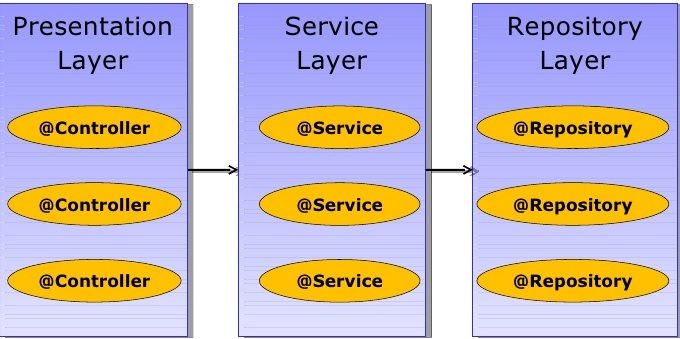
\includegraphics[width=1\textwidth]{bilder/SpringLayers} 
\caption[Der Grafik \url{http://image.slidesharecdn.com/springsourceusi2009v3-0-090702135517-phpapp01/95/developing-modular-java-applications-13-728.jpg?cb=1246543977} nachempfunden]{Konzept einer Spring-Anwendung}
\end{figure} 

Gleichzeit stellt Spring-Boot auch direkt einen Container für die Webapplikation zur Verfügung. Das bedeutet, dass die Programmierung sich komplett mit der REST-API und ihren Funktionalitäten beschäftigen kann und nur sehr wenig Zeit für die Konfiguration des Web-Servers verbraucht wird.

Sollte Konfiguration nötig sein so findet diese zu großen Teilen außerhalb des Codes statt. In dem Projekt kann eine Datei mit dem Namen ``application.properties'' hinterlegt werden. Hier können dann mehrere Sachen eingestellt werden, wie zum Beispiel der Port unter dem der Server laufen soll.\\

\begin{minipage}{\textwidth}
\emph{Konfiguration des Server-Ports}
\begin{lstlisting}
spring.server.port=8080
\end{lstlisting} 
\end{minipage}

\subsection{Spring Data JPA}

\emph{\glqq   
Implementing a data access layer of an application has been cumbersome for quite a while. Too much boilerplate code has to be written to execute simple queries as well as perform pagination, and auditing. Spring Data JPA aims to significantly improve the implementation of data access layers by reducing the effort to the amount that’s actually needed. As a developer you write your repository interfaces, including custom finder methods, and Spring will provide the implementation automatically.
\grqq} \footnote{http://projects.spring.io/spring-data-jpa/} \\

Bei Spring Data JPA (im nachfolgenden nur noch als JPA bezeichnet) handelt es sich um eines der Projekte aus dem Spring-Ökosystem welches in beinahe jedem Spring Projekt heutzutage genutzt wird. Das Hauptziel des Projektes ist die Reduktion von redundantem Code welcher in beinahe jedem Projekt für den Zugriff auf Datenbanken benötigt wird. Zusätzlich werden benötigte Querys zur Abfrage von Daten automatisch generiert, der Nutzer muss lediglich ein Interface mit vorgegebenen Methodennamen erzeugen. \\

Um mit dem Aufbau der Datenbankverbindung zu beginnen benötigt JPA als erstes die Information unter welcher Adresse die Datenbank erreichbar ist. Dies wird in der application.properties angegeben \\

\begin{minipage}{\textwidth}
\emph{Konfiguration der Datenbankverbindung}
\begin{lstlisting}
spring.datasource.url=jdbc:mysql://localhost:3306/bachelor
spring.datasource.username=root
spring.datasource.password=root
\end{lstlisting} 
\end{minipage}

Nach dem JPA nun die Verbindung mit der Datenbank aufbauen kann muss definiert werden wie die Datenbank-Entitäten in Java-Objekte umgewandelt werden und in welchen Tabellen sie sich befinden. In JPA wird dies dadurch umgesetzt, dass für jede Entität eine Klasse angelegt wird in der durch Annotationen festgelegt wird wie die Daten in das Objekt geladen werden. \\

\begin{minipage}{\textwidth}
\emph{Beispiel für eine Datenbank-Entität}
\begin{lstlisting}
@Entity
@Table(name="scripts")
public class ScriptEntity implements Serializable{

	@Id
	@GeneratedValue(strategy= GenerationType.IDENTITY)
	private Integer id;
	
	@Column(nullable=false, name="name")
	private String name;
	
	@Column(nullable=false, name="variablescript")
	private String variableScript;
	
	@Column(nullable=false, name="solutionscript")
	private String solutionScript;

	@Column(nullable=false, name="mathjaxscript")
	private String mathjaxScript;
	
	/*Getter/Setter/Konstruktor*/
}
\end{lstlisting}
\end{minipage}

Zu guter Letzt muss ein Interface erzeugt werden, welches definiert was für Querys zur Verfügung stehen. Um das zu realisieren wird ein Interface erzeugt, welches die Querys erzeugt indem es bei der Benennung der Methoden bestimmten Konventionen folgt. Wichtig ist hierbei, dass es das bereits gegebene Interface CrudRepository erweitern muss. Dadurch wird es von JPA erkannt und einige Funktionalität direkt gegeben (wie zum Beispiel findAll, save und delete).
Um nun eigene Querys hinzufügen gibt es zwei Möglichkeiten. Entweder über eine Annotation oder über die Benennung der Funktion. \\

\begin{minipage}{\textwidth}
\emph{Beispiel für eigene Querys}
\begin{lstlisting}
public interface ScriptRepository extends CrudRepository<ScriptEntity, Integer> {

	public ScriptEntity findByName(String name);
	
	@Query("SELECT p FROM ScriptEntity s WHERE s.name = :name")
	public ScriptEntity customQuery(@Param("name")String name);
}
\end{lstlisting}
\end{minipage}

Nachdem das Interface deklariert wurde kann es jederzeit über den Dependency-Injektor geholt und genutzt werden.\\

\begin{minipage}{\textwidth}
\emph{Beispiel für die Nutzung des Repositorys}
\begin{lstlisting}

	@Autowired
	private ScriptRepository scriptRepository;
	
	public List<ScriptEntity> getAllScriptEntities() {
		return scriptRepository.findAll();
	}
	
}
\end{lstlisting}
\end{minipage}

\subsection{Bootstrap}

\emph{\glqq   
Bootstrap ist ein anpassungsfähiges und zuerst für mobile Geräte entwickeltes Framework. Egal, wie gut du dich auskennst, kannst du damit einfacher und schneller kleine wie große Projekte entwickeln, die auf Geräten in allen erdenklichen Formen funktionieren.
\grqq} \footnote{http://holdirbootstrap.de//} \\

Aus der heutigen Welt der Webentwicklung ist Bootstrap kaum wegzudenken. Durch die leichte Entwicklung für alle vorhandenen Formate und Endgeräte hat es sich als äußerst robust herausgestellt wenn es um die schnelle Entwicklung von Webseiten geht. \\
Gleichzeitig bietet es ein großes Repertoire an CSS-Klassen für alle Elemente der HTML-Entwicklung was es sogar Personen mit wenig Erfahrung im Design-Bereich ermöglicht spektakuläre Ergebnisse mit wenig Arbeit zu erzielen. \\

Da bei OpenTasks bereits durch die technische Implementation ein hoher Grad an Komplexität gegeben war konnte nicht viel Zeit für das Einarbeiten in ein komplexes CSS-Framework investiert werden, daher ist die Wahl recht schnell auf Bootstrap gefallen. Als Alternative hätte sonst Material \footnote{http://materializecss.com/} zur Auswahl gestanden. \\



\subsection{Typescript / Angular 2} \label{TS_NG2}

Bevor man sich mit der Technologie beschäftigt die benutzt wurde um das Frontend zu bauen muss man sich vorher mit einer anderen Errungenschaft der Webentwicklung auseinander setzen. Typescript. \\

\emph{\glqq   
TypeScript is a free and open-source programming language developed and maintained by Microsoft. It is a strict superset of JavaScript, and adds optional static typing and class-based object-oriented programming to the language. \\
TypeScript is designed for development of large applications and transcompiles to JavaScript. As TypeScript is a superset of JavaScript, any existing JavaScript programs are also valid TypeScript programs.
\grqq} \footnote{https://en.wikipedia.org/wiki/TypeScript} \\

Besonders für Entwickler welche aus der Welt der stark-typisierten Programmierwelt kamen war TypeScript ein großer Fortschritt. Durch die Möglichkeit Variablen stark zu typisieren entstand die Möglichkeit Schnittstellen klarer zu definieren. Gleichzeitig wurden die bestehenden Möglichkeiten Entwicklungsumgebungen mit Auto-Vervollständigung auszustatten verbessert. \\
Die Vorteile die sich daraus für die Entwicklung sind recht eindeutig: Eine Beschleunigung der Entwicklung, während die Testbarkeit vereinfacht wird und Fehler besser vermieden werden können. Kurz gesagt: Bessere Software in weniger Zeit. \\

Was für die Anwendung relativ früh klar war war, dass es sich um eine Single Page Application (kurz SPA) handeln sollte. Doch was genau ist das und wieso sollte es verwendet werden? \\


\emph{\glqq   
Als Single-Page-Webanwendung (englisch single-page application, kurz SPA) oder Einzelseiten-Webanwendung wird eine Webanwendung bezeichnet, die aus einem einzigen HTML-Dokument besteht und deren Inhalte dynamisch nachgeladen werden. Diese Art von Web-Architektur steht im Gegensatz zu klassischen Webanwendungen, die aus mehreren, untereinander verlinkten HTML-Dokumenten bestehen. Hierdurch wird allerdings die Grundlage geschaffen, eine Webanwendung in Form einer Rich-Client- bzw. Fat-Client-Verteilung zu entwickeln. Eine verstärkte clientseitige Ausführung der Webanwendung ermöglicht eine Reduzierung der Serverlast sowie die Umsetzung von selbstständigen Webclients, die beispielsweise eine Offline-Unterstützung anbieten.
\grqq} \footnote{https://de.wikipedia.org/wiki/Single-Page-Webanwendung} \\

Warum also eine Single-Page-Application? Der Hauptvorteil liegt darin, dass bei dem Initialisieren der Seite fast alle benötigten Informationen geladen werden, somit fallen die Ladezeiten nach der ersten Initialisierung sehr gering aus. Das sorgt insbesondere bei Nutzern von mobilen Endgeräten für eine bessere User-Experience, da bei diesen (bedingt durch schwächere Prozessoren) die Ladezeiten besonders ins Gewicht fallen. Gleichzeitig reduzieren sich die Anforderungen an den Webserver, da der Content nur ein einziges Mal ausgeliefert werden muss. Lediglich durch das Abfragen einiger Daten zur Laufzeit (wie zum Beispiel das Erhalten einer neuen Aufgabe) wird der Server nach dem Ausliefern der Webseite kontaktiert.\\

Nachdem nun evaluiert wurde, dass eine SPA ein Gewinn ist also die Frage nach dem Framework / der Library um das umzusetzen. Im Raum stehen zwei Varianten. Zum einen ReactJS (welches seit längerem existiert und weit bekannt ist) oder das vor kurzem aus der Beta gekommene Angular2. \\
Direkt zu sagen ist, dass Angular 2 von Haus aus mit TypeScript gebaut ist. Das bedeutet bester TypeScript-Support bei der Entwicklung von Angular 2, was bei ReactJS nur teilweise der Fall ist und viele Varianten wie man am besten mit ReactJS und Typescript arbeitet sich widersprechen da keine klare Konvention herrscht. \\
Zusätzlich implementiert Angular 2 eine bessere Trennung der verschiedenen Komponenten. Während in ReactJS HTML und Javascript Code in der selben Klasse stehen werden in Angular 2 klare Mechanismen aufgezeigt wie diese sauber zu trennen und in verschiedenen Dateien abzulegen sind. Was gleichzeitig auch einer der Nachteile von Angular 2 ist. Dadurch, dass HTML und Script sauber getrennt werden ist es schwerer die Script-Variablen im HTML zu referenzieren und alle Namen im Kopf zu behalten ohne die zweite Datei irgendwo geöffnet zu haben. \\

Bei Angular 2, sowie ReactJS handelt es sich standardmäßig um Technologien bei denen ``Client-Side Rendering'' betrieben wird. Das beudetet, dass vom Server alle Dateien ausgeliefert werden die benötigt werden. Der Client nimmt diese entgegen, rendert die einzelnen Komponenten und fügt diese korrekt zusammen. Das bedeutet, dass die Last des Rendering auf den Client übertragen wird. Das bedeutet weniger Aufwand für den Server, gleichzeitig aber eine bessere Performanz für den Server (da dieser nicht selber rendern muss). Was bei Angular 2 aber auch unterstützt wird ist die Möglichkeit auf der Seite des Server zu rendern. Das bedeutet wenn man  die Ladezeiten auf dem Client reduzieren will und einen performanten Server zur Hand hat ist dies die korrekte Lösung. Möglich ist dies durch eine die kürzlich heraus gekommene Bibliothek Angular Universal  \footnote{https://universal.angular.io/}. \\

Ein Feature welches ebenfalls beide Bibliotheken implementieren ist das sogenannte ``Two-Way-Binding''. Bei dem Two-Way-Binding wird eine Variable, welche in der View genutzt wird mit einer Variable aus dem Model verknüpft. Ein klassisches Beispiel dafür sind Textfelder. Wenn der Nutzer eine Eingabe betätigt wird dies ebenfalls an das Model weitergeleitet, welches daraufhin die zugehörige Variable erneuert. Gleichzeitig wird bei Veränderung der Variable im Model die View geupdatet. So kann man zum Beispiel ein Knopf der für einen Reset des Textfeldes verantwortlich ist einfach die Variable im Model ändern, die View wird automatisch erneuert. \\

Am Ende fiel die Wahl auf Angular 2, auf Grund der oben genannten Vorteile zusätzlich dazu, dass hinter Angular 2 ein Team von Entwicklern steht welche Erfahrungen aus einem vorherigen Projekt (AngularJS) gezogen haben um daraus von neu an ein komplett neues Framework zu erstellen welches aus den Problemen der alten Version gelernt hat und diese ausgemerzt hat.

\subsection{SocketIO}

Es stand bereits sehr früh klar, dass Daten vom Server zum Client übertragen werden müssen um den aktuellen Stand der Aufgaben für die Übersicht des Administrators aktuell zu halten. Früher hätte man dafür Long Polling verwendet, doch heute gibt es eine Technologie, welche erheblich besser für diesen Zweck geeignet ist: Websockets. \\

TODO: Mehr Long Polling erklären

\emph{\glqq   
WebSockets ist eine fortschrittliche Technologie welche es möglich macht eine interaktive Kommunikations-Session zwischen dem Browser des Benutzers und dem Server herzustellen. Mit dieser API können Sie Nachrichten zum Server senden und ereignisorientierte Antworten erhalten ohne beim Server die Antwort abzufragen.
\grqq} \footnote{https://developer.mozilla.org/de/docs/WebSockets} \\


Für dieses Protokoll gibt es inzwischen etliche Implementierungen (PubNub, WS, uWebSockets um nur einige zu nennen), da für dieses Projekt am wichtigsten war eine zuverlässige Lösung zu haben fiel die Entscheidung am Ende auf socket.io, da es ein Projekt ist welches schon sehr lange genutzt, gewartet und weiterentwickelt ist. Daher ist bei einem so erfahrenen Entwicklerteam zu rechnen, dass es recht reibungslos funktioniert und auch zukünftige Versionen stabil und performant sind.

\subsection{JSON Web Tokens} \label{JWT}

Wenn man im Web-Bereich Anwendungen entwickelt gibt es einne Abschnitt welcher fast immer relevant ist: Die Authentifizierung. Daher ist dieser Bereich inzwischen auch so vielschichtig und es gibt enorm viele Möglichkeiten und Verfahren Authentifizierung erfolgreich umzusetzen. Als Verfahren welches wohl am längsten dabei ist gibt es zum Beispiel ``Basic Auth''. Hierbei wird bei jeder Anfrage im Header der Nutzername und das Passwort übertragen. Dieses wird auf Server Seite überprüft und bei Korrektheit die Daten ausgeliefert. Der Vorteil ist eine sehr einfache Logik, allerdings muss der Server bei jeder Anfrage die Korrektheit von Nutzername und Passwort überprüfen, sowie eventuelle Daten die mit dem Nutzer in Verbindung stehen aus der Datenbank extrahieren. \\

Zwei Ansätze die sich relativ ähneln sind Token und Cookie Authentication. Bei beiden wird ein Objekt generiert welches von dem Client als Authentifizerungs-Objekt bei jeder Anfrage mitgeschickt wird. Der Unterschied ist, dass Cookies direkt im Browser gespeichert werden, während die Speicherung von Tokens vom Programmierer selber entwickelt werden muss (und dann meistens im RAM gehalten werden). \\

Am Ende ist die Wahl auf JSON Web Tokens(JWT) gefallen. Zusätzlich zu den Authentifizierungsmöglichkeiten beinhaltet JWT die Möglichkeit Nutzdaten im Token mitzuschicken. Das bedeutet, dass der Nutzer nach der Authentifizierung Daten erhalten kann welche für die gesamte Nutzung der Anwendung wichtig sind, wie zum Beispiel welche Rolle er erhalten hat und welche Rechte damit verbunden sind. 

\subsection{MathJax}

Da innerhalb der folgenden Seiten der Begriff MathJax mehrfach verwendet wird, wird hier einmal darauf eingegangen was genau damit gemeint ist. \\

Bei MathJax \footnote{https://www.mathjax.org/} handelt es sich um eine JavaScript-Bibliothek die im Jahre 2004 von Davide Cervone ins Leben gerufen wurde. Das Ziel dieser Bibliothek ist die Darstellung von mathematischen Formeln in jedem Browser ohne sich Sorgen um Kompatibilität zu machen. \\
Dies funktioniert indem auf der Webseite innerhalb eines HTML-Elements ein Text eingetragen wird, welcher einer von mehreren Syntaxen folgt. Daraufhin wird der Bibliothek mitgeteilt, dass es die Seite scannen soll. Sollte sie Elemente finden, bei denen es sich um mathematische Formeln handelt werden diese in HTML-Elemente umgewandelt welche die Formel korrekt darstellen. \\

Innerhalb von OpenTasks wird ausschließlich die LaTex-Syntax \footnote{https://en.wikibooks.org/wiki/LaTeX/Mathematics} verwendet um mathematische Formeln darzustellen.

\chapter{Ein Rundgang durch das Frontend}

Das Frontend ist im Wesentlichen in zwei große Abschnitte geteilt - Die Ansicht des Nutzers (also die Anwendung wie sie von den Studenten gesehen wird) und die Ansicht des Administrators, welche hauptsächlich die Aufgabe hat die Anwendung zu verwalten und Einstellungen zu ändern. Daher werden diese beiden Sichten im Nachfolgenden getrennt voneinander behandelt.

\section{Die Ansicht des Nutzers}

Für den Nutzer gibt es im wesentlichen nur zwei Prozesse die wichtig sind. Die Auswahl eines Teams und die Bearbeitung der Aufgaben. Daher gibt es für diesen lediglich zwei Ansichten die für eben diese Zwecke gebaut wurden.

\subsection{Die Auswahl des Teams}

Bevor mit der Bearbeitung der Aufgaben beginnen kann ist vorher der Login-Prozess von Nöten. Der Nutzer muss dafür lediglich ein Team auswählen und dies über Knopf-Druck bestätigen. Um die Auswahl besonders für Mobiltelefone gut auszulegen ist die Auswahl über Knöpfe gewählt worden. Um die aktuelle Auswahl hervorzuheben wird das ausgewählte Team als Text über den Knöpfen dargestellt, zusätzlich wird der entsprechende Knopf mit rotem Text versehen.

\begin{figure}[htp]     % h=here, t=top, b=bottom, p=page
\centering
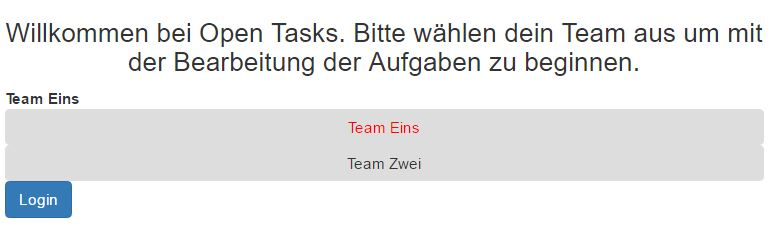
\includegraphics[width=1\textwidth]{bilder/UserLogin} 
\caption[Login für den Nutzer / Teamauswahl]{Team Auswahl für den Nutzer}
\end{figure} 

Sobald der Login Knopf betätigt wurde werden mehrere Pakete an den Server geschickt. Bei dem Ersten handelt es sich um das Erhalten des Tokens welches in Zukunft für die eindeutige Identifizierung und Authentifizierung zur Nutzung der REST-API genutzt wird. Sobald dieser Prozess beendet wurde wird die Auswahl des Teams übermittelt. Sind alle diese Prozesse erfolgreich wird auf die Bearbeitung der Aufgaben weitergeleitet. 

\subsection{Erhalten und bearbeiten der Aufgaben}

Nachdem nun die initiale Prozedur der Team-Auswahl beendet ist kommt der Student zu dem Hauptteil der Anwendung. Die Erhaltung und Bearbeitung der Aufgaben. Nach der Einwahl erscheint ein Hinweis, dass bisher keine Aufgabe gefunden wurde. Durch das Betätigen des Refresh-Button kann allerdings eine Aufgabe angefordert werden. \\
\begin{figure}[htp]     % h=here, t=top, b=bottom, p=page
\centering

\includegraphics[width=1\textwidth]{bilder/NoTask} 
\caption[Ansicht bei nicht geladener Aufgabe]{Ansicht bei nicht geladener Aufgabe}
\end{figure} 

Sollte dieser Knopf betätigt werden wird eine Anfrage an den Server gesendet, welche entweder mit dem Erhalt einer Aufgabe oder der Information, dass momentan kein Generator vorhanden ist beendet wird. \\

\begin{figure}[htp]     % h=here, t=top, b=bottom, p=page
\centering
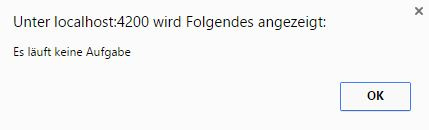
\includegraphics[width=1\textwidth]{bilder/NoTaskRunning} 
\caption[Information über keine laufende Aufgabe]{Information über keinen laufende Aufgabe}
\end{figure} 

Nach dem Erhalt einer Aufgabe beginnt die Bearbeitung. Der erhaltene Inhalt wird als mathematische Formel dargestellt, hierbei hilft die Bibliothek MathJax dabei den erhaltenen Text optisch ansprechend und mathematisch korrekt darzustellen. Der Student hat nun die Zeit die er braucht um die Aufgabe zu bearbeiten. Sollte er sich der Lösung sicher sein gibt er diese über das entsprechende Formular ein und bestätigt das Ganze mit einem Druck auf den ``Senden'' Knopf. Die Eingabe wird an den Server weitergeleitet welcher diese validiert. Für den Studenten gibt es nun drei Fälle: \\
\begin{enumerate}
\item Die Bearbeitungszeit für die Aufgabe ist abgelaufen. Der Nutzer erhält eine Informationsanzeige über den Ablauf der Zeit. Die momentan angezeigte Aufgabe wird entfernt.
\item Die Aufgabe wurde korrekt gelöst. Der Nutzer erhält eine neue Aufgabe, sowie eine Notifikation über die Korrektheit der Lösung.
\item Die Lösung war falsch. Der Nutzer wird informiert, behält aber seine momentane Aufgabe bei um eine neue Lösung anzugeben.
\end{enumerate} 

Um die Effizienz für den Studenten während der Nutzung von Open Tasks zu steigern wurden zwei weitere Features eingebaut. Bei dem Ersten handelt es sich um eine kleine Informationsanzeige wie lange die durchschnittliche Zeit beträgt bis eine Aufgabe korrekt gelöst wurde. Dies soll dem Studenten helfen seine Leistungen zu überprüfen und sich vielleicht auch mit anderen zu vergleichen. \\
Bei dem Zweiten handelt es sich um die Eingabeformulare. Je nachdem was für eine Aufgabe bearbeitet wird wird ein Formular angezeigt, welches darauf ausgelegt ist die Lösung einfach einzugeben. Eine Sache die alle gemeinsam haben ist die Validierung ob die momentane Antwort des Nutzers korrekt sein könnte und die graphische Darstellung davon (grün / rot- Färbung des Antwort Textes). Wie genau diese Validierung aussieht und welche weiteren Funktionalitäten das Formular bietet ist allerdings von Formular zu Formular unterschiedlich.

\begin{figure}[htp]     % h=here, t=top, b=bottom, p=page
\centering
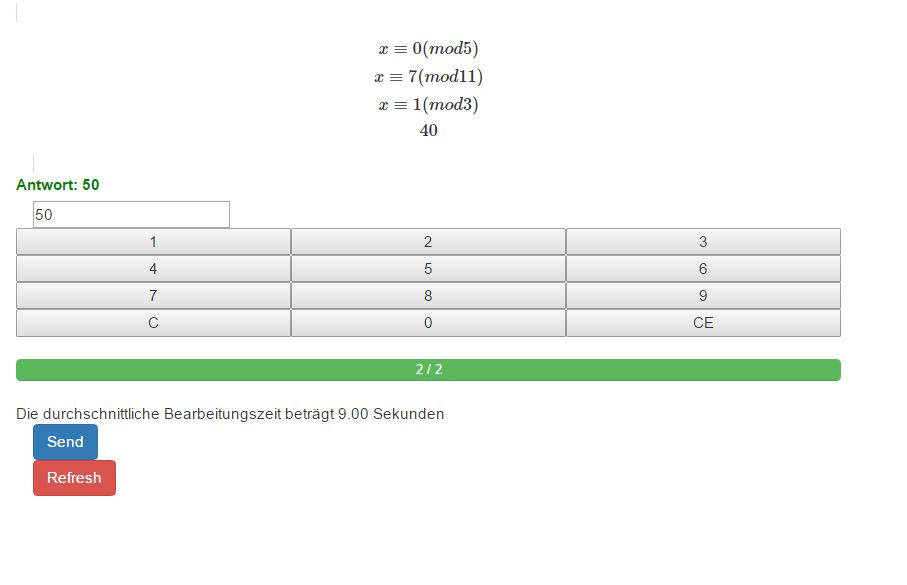
\includegraphics[width=1\textwidth]{bilder/TotalClient} 
\caption[Beispiel für eine komplette Seite zur Bearbeitungszeit]{Beispiel für eine komplette Seite zur Bearbeitungszeit}
\end{figure} 


\subsection{Die Eingabeformulare}

Insgesamt existieren fünf Eingabeformulare.
\begin{enumerate}
\item Das Textformular
\item Das Zahlenformular
\item Das Dezimalformular
\item Das Matrixformular
\item Das Bruchformular
\end{enumerate}

In diesem Kapitel werden diese genauer unter die Lupe genommen und darüber gesprochen wie genau ihre graphische Darstellung ist, sowie die Validierung ob eine Antwort korrekt sein kann und abgeschickt werden darf. \\
Die Antwort die sich am Ende von dem Formular ergibt wird zusätzlich immer über dem Formular noch einmal angezeigt. So kann der Nutzer überprüfen, dass seine Antwort dem Gewünschten entspricht. \\
Welches Formular angezeigt wird wird immer von dem Administrator der Anwendung ausgewählt, für weitere Informationen bitte im Kapitel \ref{EditGenerator} Bearbeitung der Generatoren und ihrer Hilfsmittel nachlesen.


\subsubsection{Das Textformular}

Bei dem Textformular handelt es sich um das wohl einfachste aller Formulare. Die graphische Darstellung besteht lediglich aus einer Textbox. \\
Ähnlich simpel ist ebenfalls die Validierung, es wird lediglich überprüft, dass die Antwort eine Länge von mindestens einem Zeichen hat, sodass keine leeren Antworten abgegeben werden können.

\subsubsection{Das Zahlen / Dezimalformular}

Da sich das Zahlen und das Dezimal-Formular sehr ähnelt werden sie hier gemeinsam behandelt. Da es sich bei den Nutzern von Open Tasks zu großen Teilen um mobile Endgeräte nutzen wird wurde dieses Formular mit einem speziellen Fokus auf diese entworfen.

\begin{figure}[htp]     % h=here, t=top, b=bottom, p=page
\centering
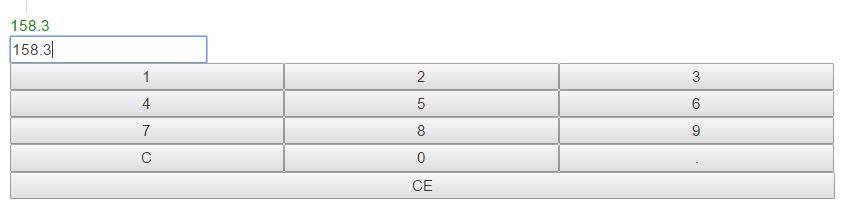
\includegraphics[width=1\textwidth]{bilder/DezimalForm} 
\caption[Das Dezimalformular]{Das Dezimalformular}
\end{figure} 

\begin{figure}[htp]     % h=here, t=top, b=bottom, p=page
\centering
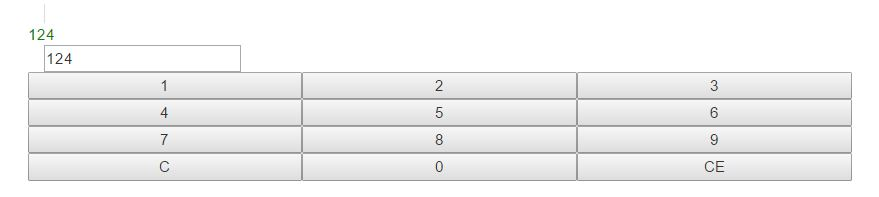
\includegraphics[width=1\textwidth]{bilder/NumberForm} 
\caption[Das Zahlenformular]{Das Zahlenformular}
\end{figure} 

Die Eingabe kann über zwei Wege erfolgen. Bei dem Ersten handelt es sich um die Eingabe der Lösung über das Textfeld. Dies ist besonders für die Nutzer von Laptops gut, da hier eine Tastatur zur Verfügung steht. \\
Für die mobilen Endgeräte wurden Knöpfe implementiert, welche bei Druck die abgebildete Zahl der Antwort hinzufügen. Außerdem gibt es noch zwei weitere Knöpfe, einen um die letzte Eingabe zu entfernen (C) und einen um das gesamte Eingabefeld zu leeren (CE). Ein Unterschied zwischen den beiden Formularen ist, dass das Dezimalformular zusätzlich einen Knopf besitzt welcher einen Punkt einfügt und es so ermöglicht Kommazahlen einzugeben. \\
Der zweite Unterschied liegt in der Validierung der Eingaben. Während bei dem Zahlenformular nur Ganze Zahlen erlaubt sind werden bei dem Dezimalformular alle reellen Zahlen angenommen.

\subsubsection{Das Matrixformular}

Für einige Aufgabentypen war es notwendig, dass der Nutzer in der Lage ist eine Matrix als Antwort einzugeben. Da dies in einem Textfeld sehr schwer ist wurde das Matrixformular entwickelt. \\

\begin{figure}[htp]     % h=here, t=top, b=bottom, p=page
\centering
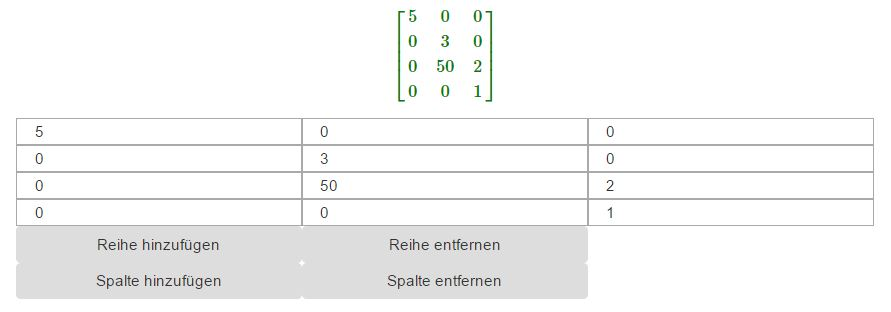
\includegraphics[width=1\textwidth]{bilder/MatrixForm} 
\caption[Das Matrixformular]{Das Matrixformular}
\end{figure} 

Bei dem Matrixformular handelt es sich um Textfelder im $ m\times n$ Format, genau wie die Matrix die erzeugt werden soll. Dabei wird die produzierte Matrix immer über dem Formular angezeigt, dabei hilft wieder die MathJax Bibliothek das Ganze optisch ansprechend aufzubereiten. \\

Ein weiterer wichtiger Einfluss bei der Erstellung des Formulars war die Tatsache, dass die Größe der Matrix nicht am Anfang bekannt ist. Zum einen liegt dies daran, dass dies ein Tipp für den Studenten sein kann (da die Größe der entstehenden Matrix unter Umständen berechnet werden muss). Andererseits liegt dies auch daran, dass es ein größerer Aufwand wäre direkt bei der Generierung festzulegen wie groß die Matrix sein soll. Dieses Problem wurde über vier Knöpfe gelöst, welche die Manipulation der Größe der Matrix erlauben, jeweils zwei für Spalten und Reihen. \\

Ein weiteres Feature welches in diesem Formular implementiert wurde ist eine automatische Korrektur der Eingabe des Nutzers. Sollte der Nutzer sich vertippen und zum Beispiel aus Versehen einen Buchstaben in eines der Felder eintippen so wird dies automatisch korrigiert indem der Buchstabe entfernt und nicht in der Lösung angezeigt wird. \\

Für die mobilen Nutzer wurde ein Knopf implementiert welcher auf eine alternative, für mobile Nutzer angepasste Sicht umschaltet. Diese ähnelt sehr der Ansicht von dem Nummernformular. Der Nutzer wählt über Knopfdruck aus welches Feld er bearbeiten will. Daraufhin wird dieses durch blaue dickere Schrift markiert. Sollte der Nutzer nun einen der nummerierten Knöpfe drücken wird der Text des Knopfes der Eingabe hinzugefügt.


\begin{figure}[htp]     % h=here, t=top, b=bottom, p=page
\centering
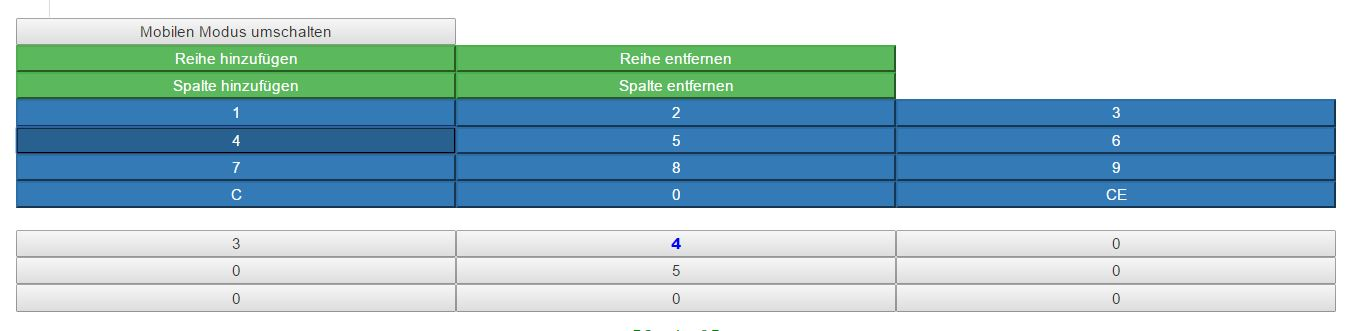
\includegraphics[width=1\textwidth]{bilder/MatrixMobile} 
\caption[Das Matrixformular]{Das Matrixformular}
\end{figure} 


\subsubsection{Das Bruchformular}

Als letztes Formular ist das Bruchformular zu erwähnen. Dies sollte jederzeit genutzt werden wenn von dem Nutzer erwartet wird einen Bruch einzugeben.

\begin{figure}[htp]     % h=here, t=top, b=bottom, p=page
\centering
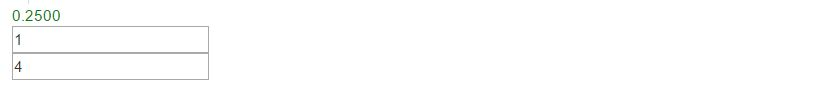
\includegraphics[width=1\textwidth]{bilder/FractureForm} 
\caption[Das Bruchformular]{Das Bruchformular}
\end{figure} 

Bei der graphischen Darstellung handelt es sich um zwei Textfelder, welche übereinander angeordnet sind. In dem oberen Feld sollte der Zähler eingetragen werden, während das untere für den Nenner vorgesehen ist. \\
Wenn der Student in beide Felder eine Zahl eingeben hat wird der Wert des Bruches berechnet. Dieser wird über den beiden Textfeldern angezeigt. \\

Die Validierung erfolgt durch ein Überprüfen des Resultats der Rechnung Zähler/Nenner. Wenn hierbei eine valide Zahl herauskommt wird dies als mögliche Antwort akzeptiert und der Antwort-Text in grün gefärbt.


\section{Die Sicht des Administrators}

Der zweite große Punkt der Anwendung war die Verwaltung und Übersicht über die Aufgaben und die Lösungen die von den Studenten abgegeben wurden. Nicht zu vergessen ist allerdings auch, dass die Aufgaben in diesem Abschnitt verwaltet und erweitert werden müssen. \\

Daher wurde diese Sektion in die Verwaltung von laufenden Aufgaben (Übersicht / Starten eines neuen Aufgaben-Generators), die Verwaltung und Erweiterung von Aufgaben (Bearbeitung der Aufgaben-Generatoren und ihren Hilfsmitteln) und das Evaluieren von Fehlerzuständen aufgeteilt (Der Fehler-Log). Die Navigation innerhalb diesem Teil der Anwendung funktioniert über die Leiste im oberen Bereich des Bildschirms. \\
\begin{figure}[htp]     % h=here, t=top, b=bottom, p=page
\centering

\includegraphics[width=1\textwidth]{bilder/NavBar} 
\caption[Navigationsleiste Admin-Bereich]{Navigationsleiste Admin-Bereich}
\end{figure} 

\subsection{Übersicht über die laufende und letzte Aufgabe}

Die während der Laufzeit wahrscheinlich am meisten genutzte Seite: Die Übersicht. Hier wird eine Oberfläche dargestellt, welche optisch aufbereitet die Daten anzeigt die von der Anwendung erzeugt werden: Die Zeit wie lange eine Aufgabe noch läuft, sowie den aktuellen Stand an richtig / falsch gelösten Aufgaben der verschiedenen Teams \\
\begin{figure}[htp]     % h=here, t=top, b=bottom, p=page
\centering
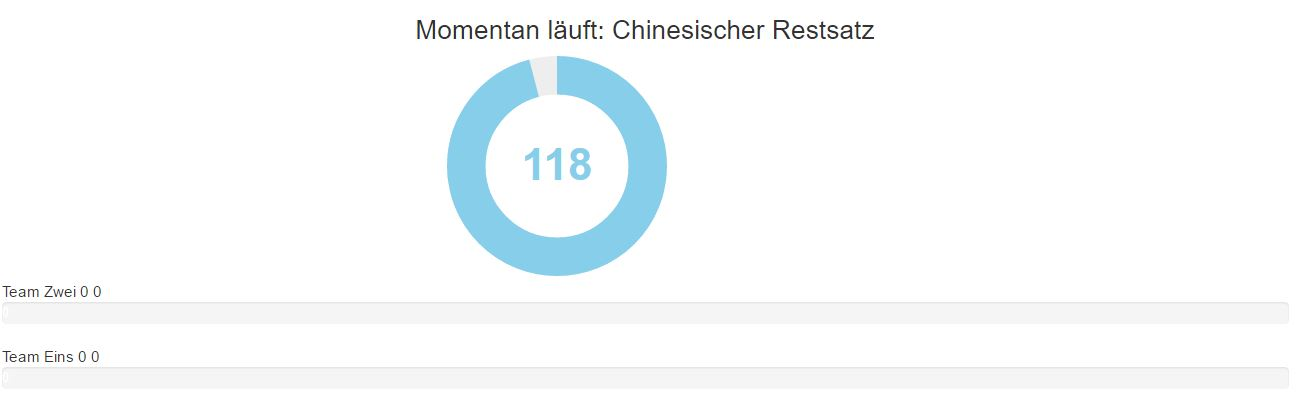
\includegraphics[width=1\textwidth]{bilder/Overview} 
\caption[Übersicht Seite während einer laufenden Aufgabe]{Übersicht Seite während einer laufenden Aufgabe}
\end{figure} 
In der obersten Zeile ist immer zu sehen welcher Generator momentan läuft (in Sekunden).

Um die Zeit die noch verbleibt darzustellen wurde die Bibliothek jQuery-Knob \footnote{https://github.com/aterrien/jQuery-Knob} verwendet, welche in Eigenarbeit in eine Angular 2 Komponente umgewandelt wurde um sie dann in die Übersicht Seite einzubetten. \\

Darunter ist abschließend der Stand der einzelnen Teams zu sehen. Die Namen der Teams werden über den Fortschrittsbalken angezeigt, welche das Verhältnis von richtig zu falsch gelösten Aufgaben darstellt. Zusätzlich ist, sobald die erste Aufgabe korrekt gelöst wurde, der absolute Stand der korrekt gelösten Aufgaben zu sehen. \\

\begin{figure}[htp]     % h=here, t=top, b=bottom, p=page
\centering
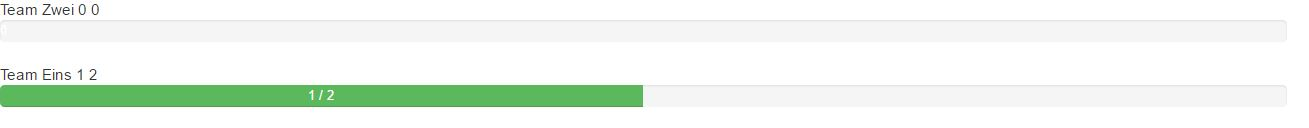
\includegraphics[width=1\textwidth]{bilder/Bars} 
\caption[Fortschrittsbalken]{Fortschrittsbalken}
\end{figure} 

Sollte die Zeit der Bearbeitung auslaufen ändert sich die Ansicht auf der Seite. Die Zeitanzeige verschwindet, und der Name des laufenden Generators wird mit der Info-Meldung ersetzt, dass zur Zeit keine aktive Aufgabe läuft. Die Anzahl der richtig und falsch gelösten Aufgaben der vergangenen Aufgabe wird allerdings weiterhin korrekt angezeigt und kann ausgewertet oder mit den Studenten besprochen werden.

\begin{figure}[htp]     % h=here, t=top, b=bottom, p=page
\centering
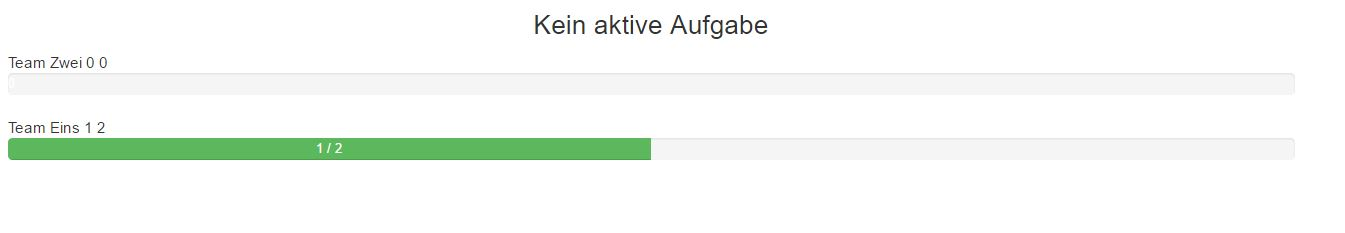
\includegraphics[width=1\textwidth]{bilder/TaskOver} 
\caption[Übersicht nach Ende der Aufgabe]{Übersicht nach Ende der Aufgabe}
\end{figure} 


\subsection{Starten eines neuen Aufgaben-Generators}

Damit das Programm in der Vorlesung genutzt werden kann reicht es allerdings nicht nur den Stand der laufenden Aufgabe anzuzeigen. Es ist ebenfalls notwendig einen neuen Generator starten zu können. \\
Dafür wurde ein Tab eingerichtet welcher unter dem Namen ``Neuen Generator starten'' erreichbar ist.
Auf dieser Seite gibt es zwei verschiedene Ansichten, die je nach Status des Programmes gezeigt werden. \\

Bei der ersten Ansicht handelt es sich um die Ansicht die gezeigt wird wenn aktuell kein Generator am Laufen ist. \\

\begin{figure}[htp]     % h=here, t=top, b=bottom, p=page
\centering
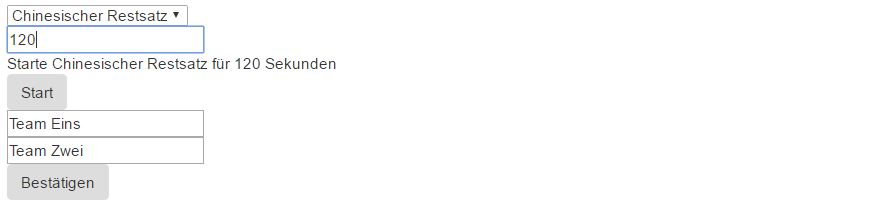
\includegraphics[width=1\textwidth]{bilder/StartNew} 
\caption[Starten eines neuen Aufgaben-Generators]{Starten eines neuen Aufgaben-Generators}
\end{figure} 

Die Ansicht besteht aus zwei Teilen. Der untere Teil besteht aus der Benennung der existierenden Teams. Der Administrator ist hier in der Lage in zwei Textfeldern die gewünschten Namen einzugeben. Danach bestätigt er die Eingabe durch Knopfdruck. Daraufhin werden die neuen Namen an den Server übertragen, welche diese nun für alle folgenden Generatoren verwenden wird. \\

\begin{figure}[htp]     % h=here, t=top, b=bottom, p=page
\centering

\includegraphics[width=1\textwidth]{bilder/StartDropDown} 
\caption[Auswahl-Menü für den zu startenden Generator]{Auswahl-Menü für den zu startenden Generator}
\end{figure} 

Bei der Auswahl welcher Generator gestartet werden soll wurde ein Drop-Down zur Auswahl des Generators gewählt. Die Namen aller erstellten Generatoren wird vom Server geholt und dann für die Befüllung der einzelnen Optionen genutzt.\\
Sollte der Start Knopf gedrückt werden ohne, dass ein Option ausgewählt wurde so erscheint eine Benachrichtigung für den Nutzer dies bitte zu korrigieren, selbiges geschieht bei einer ungültigen Angabe für die Laufzeit des Generators. \\

\begin{figure}[htp]     % h=here, t=top, b=bottom, p=page
\centering

\includegraphics[width=1\textwidth]{bilder/InvalidTime} 
\caption[Anzeige nach Drücken Start-Knopfes bei invalider Zeitangabe]{Anzeige nach Drücken Start-Knopfes bei invalider Zeitangabe}
\end{figure} 
 

Sollte aber bereits ein Generator gestartet sein wird eine andere Sicht gezeigt. Der Nutzer wird darüber informiert, dass bereits Aufgaben generiert werden. Zusätzlich wird der Name des momentan laufenden Generator angezeigt.\\
Wenn der Administrator sich nun entscheiden sollte die Aufgabe vorzeitig zu beenden (zum Beispiel weil es sich um den falschen Generator handelt oder er entschieden hat, dass die Bearbeitungszeit früher beendet wird) kann er dies durch das Drücken des ``Anhalten''-Knopfes tun.


\begin{figure}[htp]     % h=here, t=top, b=bottom, p=page
\centering

\includegraphics[width=1\textwidth]{bilder/TaskRunning} 
\caption[Anzeige bei bereits laufendem Generator]{Anzeige bei bereits laufendem Generator}
\end{figure}


\subsection{Bearbeitung der Helper-Funktionen} \label{EditGenerator}

Es war von Anfang an klar, dass es Funktionalität gab die für mehrere Aufgaben-Generatoren benötigt werden würde. Daher wurden die Helper-Funktionen eingeführt. Bei diesen handelt es sich um Funktionen welche erstellt werden und dann global verfügbar sind. Dadurch wird die Menge an überflüssigem Code der in jedem Generator erzeugt wird reduziert.

Bei den Helper-Funktionen handelt es sich um Funktionen, welche über den Tab ``Helper-Funktionen bearbeiten'' erstellt und bearbeitet werden können. \\

\begin{figure}[htp]     % h=here, t=top, b=bottom, p=page
\centering
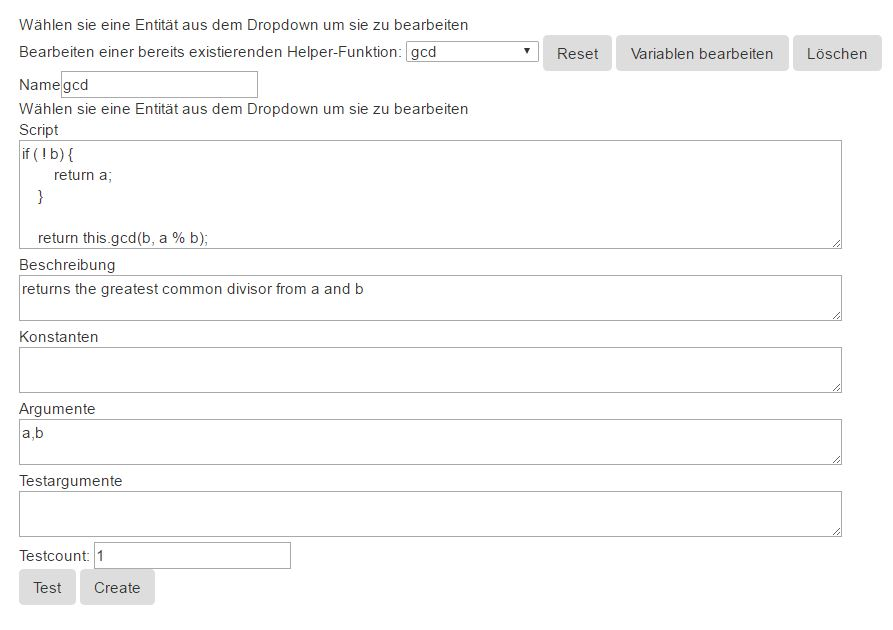
\includegraphics[width=1\textwidth]{bilder/EditHelper} 
\caption[Ansicht zur Bearbeitung einer Helper-Funktion]{Ansicht zur Bearbeitung einer Helper-Funktion}
\end{figure} 

Bevor man mit der Bearbeitung beginnt muss festgelegt werden ob es sich bei dem Skript um ein ``Variablen'' oder ein ``MathJax'' Skript handelt. Der Unterschied besteht darin, dass Variablen-Skripte dafür genutzt werden Variablen zu erzeugen, während MathJax-Skripte dabei helfen Variablen in valide MathJax-Syntax umzuwandeln.

Um mit der Bearbeitung zu beginnen muss entweder eine zu bearbeitende Entität über das Dropdown-Menü ausgewählt oder ein Name eingegeben werden. Sobald dies erledigt ist müssen die anderen Felder ausgefüllt werden. Pflicht ist hierbei nur das Skript, sowie die Argumente die das Skript benötigt. Es wird allerdings empfohlen eine Beschreibung hinzuzufügen. Dies hilft dabei sich an die Funktionalität des Skriptes zu erinnern sollte man dies in Zukunft vergessen. \\

Sollte das Skript Konstanten benötigen können diese ebenfalls in der dafür vorgesehenen Spalte eingetragen, allerdings ist hier darauf zu achten, dass die Namen der Konstante nicht mit den Konstanten von anderen Helper-Funktionen kolidieren.

\begin{figure}[htp]     % h=here, t=top, b=bottom, p=page
\centering
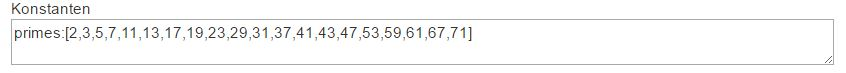
\includegraphics[width=1\textwidth]{bilder/ConstantExample} 
\caption[Beispiel zur Erstellung einer Konstanten]{Beispiel zur Erstellung einer Konstanten}
\end{figure} 

Sollte die Erstellung des Skriptes fertig sein kann getestet werden ob die erwarteten Ergebnisse produziert werden. Dafür muss der Administrator eingeben mit welchen Argumenten die Funktion aufgerufen werden soll und daraufhin den Test-Knopf betätigen. Dies stößt einen Prozess an der die Funktion in validen Javascript-kompiliert. \\

\emph{Beispiel für eine transpilierte Funktion}
\begin{lstlisting}

gcd:function(a,b){
if ( ! b) {
        return a;
    }

    return this.gcd(b, a % b);}, 
}
\end{lstlisting}

Diese Funktion wird an die global verfügbaren Objekte gehängt, Funktionen die bei der Erstellung von Variablen helfen an das ``vf''-Objekt, Funktionen die die Erstellung von MathJax erleichtern an das ``mj''-Objekt. Auf diese Objekte wird bei der Bearbeitung der Aufgaben-Generatoren noch einmal näher eingegangen. \\

Sobald der Transpilierungs-Prozess abgeschlossen ist wird die gerade erstellte Funktion mit den eingegeben Argumenten aufgerufen. Das Ergebnis wird daraufhin auf der Seite angezeigt um sich zu vergewissern, dass es den Erwartungen entspricht.  Wenn das Skript einen zufälligen Faktor besitzt ist es möglich den Test mehrere Male laufen zu lassen. Die genaue Anzahl kann in dem Feld ``TestCount'' angegeben werden. \\

Wenn nun alle Tests den Erwartungen entsprechen und das Ergebnis zufrieden stellend ist besteht die letzte Aufgabe darin es zu persistieren. Dafür wurde ein Knopf neben dem Test-Knopf eingefügt welcher die Anfrage an den REST-Server stellt. \\

\subsection{Bearbeitung der Aufgaben-Generatoren}

Nachdem die Helper-Funktionen bearbeitet und erstellt werden können kann man sich nun dem Hauptpunkt zuwenden: Den Aufgaben-Generatoren. Die Bearbeitung wird über den Tab ``Generator bearbeiten'' gestartet. \\

\begin{figure}[htp]     % h=here, t=top, b=bottom, p=page
\centering
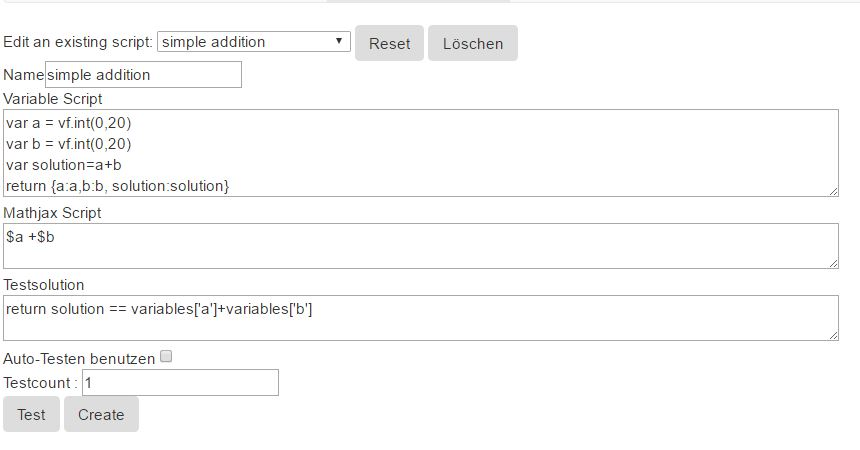
\includegraphics[width=1\textwidth]{bilder/EditScript} 
\caption[Ansicht zur Bearbeitung einer Helper-Funktion]{Ansicht zur Bearbeitung einer Helper-Funktion}
\end{figure} 

Ähnlich wie bei den Helper-Funktionen kann entweder ein bestehendes Skript über das Dropdown-Menü gewählt und editiert werden, ansonsten kann direkt mit der Editierung angefangen werden. \\

Bevor allerdings näher auf die Erstellung der drei verschiedenen Skripte eingegangen wird sollte zuerst die Nutzung der Helper-Funktionen näher erläutert werden. \\

Jede dieser Funktionen wurde einem bestimmten Objekt zugeordnet, entweder dem ``vf''(Variable-Functions) oder dem ``mj'' (MathJax) Objekt, je nachdem für welche Kategorie von Aufgabe sie erstellt wurden. Je nachdem welches der Textfelder nun fokussiert wird wird  neben ihnen angezeigt welche Funktionen vorhanden sind, sowie welche Parameter benötigt werden. Wenn nähere Informationen benötigt werden so lässt sich durch Bewegung der Maus über den Namen der Funktion die Beschreibung lesen.\\

\begin{figure}[htp]     % h=here, t=top, b=bottom, p=page
\centering
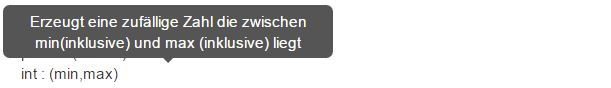
\includegraphics[width=1\textwidth]{bilder/MouseOver} 
\caption[Popup bei Bewegen der Maus über einen Funktionsnamen]{Popup bei Bewegen der Maus über einen Funktionsnamen}
\end{figure} 

Bei der Erstellung eines Aufgaben-Generators existieren drei Felder von denen alle Pflicht sind. \\

Bei dem Variablen-Skript handelt es sich um das Skript welches die Variablen erzeugt. Dadurch, dass in diesem Skript Funktionen genutzt werden können, welche in der Lage sind zufällig Werte zu generieren wird gewährleistet, dass verschiedene Aufgaben erzeugt werden (auch wenn die Chance besteht, dass zwei generierte Aufgaben sich gleichen, diese Chance sinkt jedoch je größer der Zahlenraum der generierten Werte ist). Dieses Skript muss ein JSON-Objekt zurück geben welches alle Werte enthält die für die graphische Darstellung, sowie die Validierung der Lösung von Nöten sind. \\
Um die Erstellung von diesem Skript zu erleichtern wurde ein Transpiler-Feature eingebaut. Dieses sorgt dafür, dass jeder Code der von zwei Prozent-Zeichen umgeben wird zu einem Funktionsblock umgesetzt wird. Dies hilft dabei Code zu schreiben bei dem Funktionen aufgerufen werden die wiederum Funktionen als Parameter benötigen.\\


\emph{Code vor der Transpilierung}
\begin{lstlisting}
var mod1 = vf.prime(5)
var mod2= vf.dif(%vf.prime(5)%, mod1)
\end{lstlisting}

\emph{Code nach der Transpilierung}
\begin{lstlisting}
var mod1 = vf.prime(5)
var mod2= vf.dif(function(){return vf.prime(5)}, mod1)
\end{lstlisting}


Bei der zweiten Kategorie handelt es sich um die graphische Darstellung. Der hier erzeugte Wert wird nachher von der MathJax-Bibliothek interpretiert und muss daher dessen Syntax folgen. Um die von dem ersten Skript erzeugten Werte zu nutzen werden diese über Dollar-Zeichen referenziert. So wird \$a immer durch den Wert ersetzt der für a errechnet wurde.  Wenn hier Funktionen aufgerufen werden müssen, so sind diese immer durch Prozent-Zeichen von dem Rest des MathJax-Strings zu trennen. Der Transpiler erkennt diese und kann so den Code in gültigen JavaScript-Code übersetzen \\

\begin{figure}[htp]     % h=here, t=top, b=bottom, p=page
\centering
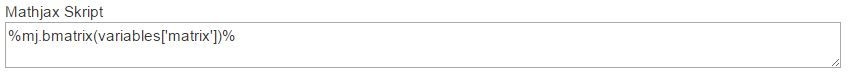
\includegraphics[width=1\textwidth]{bilder/MathJaxPreTrans} 
\caption[MathJax-Skript vor der Transpilierung]{MathJax-Skript vor der Transpilierung}
\end{figure} 

\emph{Skript nach der Transpilierung}
\begin{lstlisting}
return "$$ "+mj.bmatrix(variables['matrix'])+" $$"
\end{lstlisting}
Das von dem ersten Skript erzeugte JSON-Objekt ist im Code unter dem Namen ``variables'' referenzierbar. \\

Als letztes Skript wird die Validierung der Antworten des Nutzers benötigt. Diese Skript muss als Rückgabe einen Boolean Wert produzieren, welcher für die Korrektheit der übergebenen Antwort steht (also true bei korrekt und false bei falsch). \\
Während der Validierung der Antwort stehen dem Skript zwei Variablen zur Verfügung.\\
\begin{enumerate}
\item Das Variablen-Skript erzeugte JSON-Objekt, unter dem Namen ``variables''.
\item Die vom Nutzer eingegebene Antwort, ein String unter dem Namen userinput''.
\end{enumerate}

Diese können nun dafür genutzt werden um die Nutzereingabe zu validieren und den korrekten Wert zurück zugeben. Für diese Skript gelten die selben Transpilierungs-Regeln wie für das Variablen-Skript.


\subsection{Das Teilen von Aufgaben}

Es ist nun also möglich Aufgaben-Generatoren, sowie unterstützende Funktionalität zu erzeugen. Doch was ist wenn man keinen Generator selber schreiben will, oder ihn von einer Instanz von Open Tasks auf eine andere übertragen will? \\
Bisher war dies nur möglich indem man Teile der Datenbank manuell kopiert, doch konnte dies keine dauerhafte Lösung sein. Daher wurde das hoch und runter laden von Entitäten eingeführt.
\subsubsection{Entitäten runterladen}


Wenn man die Seite betritt sieht man ein recht simples Interface. Man wird über die Funktionsweise der Seite informiert. Danach sieht man alle Generatoren / MathJax-, sowie Variablen-Funktionen aufgelistet. \\

\begin{figure}[htp]     % h=here, t=top, b=bottom, p=page
\centering
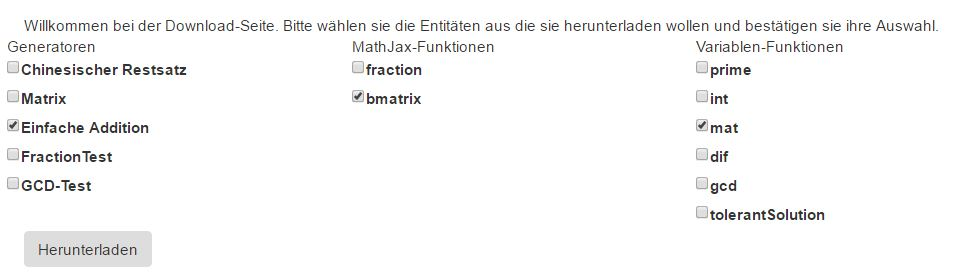
\includegraphics[width=1\textwidth]{bilder/DownloadEntities} 
\caption[Seite zum herunterladen von Entitäten]{Seite zum herunterladen von Entitäten}
\end{figure} 


Will man eine Entität zum Download auswählen muss man lediglich auf die zugehörige Checkbox oder den Text neben ihr drücken. Sobald die Auswahl beendet ist und der Herunterladen Knopf betätigt wurde wird eine Datei heruntergeladen. Diese Datei enthält alle eben gewählten Entitäten. Als Speicherformat wurde hierfür JSON gewählt, da dies nativ von JavaScript unterstützt wird und ohne Probleme gelesen und manipuliert werden kann. Diese Datei kann nun auf jedem gewünschten Weg verteilt und genutzt werden.


\subsubsection{Entitäten hochladen}

Doch wenn es möglich ist die Entitäten herunterzuladen muss es auch einen Weg geben diese wieder hoch zu laden und so in das Repertoire von Open Tasks zu integrieren. Dies wird über den Tab ``Entitäten hochladen'' getan. \\

\begin{figure}[htp]     % h=here, t=top, b=bottom, p=page
\centering

\includegraphics[width=1\textwidth]{bilder/UploadNoSelect} 
\caption[Seite zum hochladen von Entitäten vor Auswahl einer Datei]{Seite zum hochladen von Entitäten vor Auswahl einer Datei}
\end{figure} 

Diese Seite sieht bei Betreten sehr leer aus. Lediglich die Bitte eine Datei über den zugehörigen Knopf auszuwählen, sowie ein kleiner Info-Text sind zu sehen. Auf Knopfdruck öffnet sich ein Dialog zum Selektieren einer Datei. \\
Sobald eine Datei ausgewählt wurde wird diese analysiert. Bei diesem Prozess werden alle Generatoren, sowie alle Helper-Funktionen nach unerlaubten Funktionen durchsucht. Sollten welche vorhanden sein wird der Prozess mit der Warnung, dass unerlaubte Funktionen gefunden wurden abgebrochen. \\

Sollten allerdings nur erlaubte Funktionen entdeckt werden wird der Prozess fortgesetzt. Die entdeckten Entitäten werden mit denen die in der Datenbank existieren abgeglichen. Dies läuft in zwei Schritten ab.\\

1. Die Namen der neuen Entitäten werden mit denen der Datenbank verglichen. Sollte eine gefunden werden welche den selben Namen wie eine Datenbank-Entität besitzt wird diese vorgemerkt.\\

2. Die vorgemerkten Entitäten werden im Detail verglichen. Während vorher nur die Namen abgeglichen wurden, werden jetzt alle fraglichen Entitäten komplett aus der Datenbank geladen und an den Client geschickt. Dieser vergleicht nun die beiden Datensätze ins Detail ob sie komplett identisch sind. Sollte hierbei ein Unterschied entdeckt werden wird die Entität als ``Konflikt mit der Datenbank'' markiert. Ansonsten werden sie als äquivalent mit dem Datenbank-Eintrag markiert. \\

Wenn dieser Prozess abgeschlossen ist wird dem Nutzer das Ergebnis angezeigt.

\begin{figure}[htp]     % h=here, t=top, b=bottom, p=page
\centering
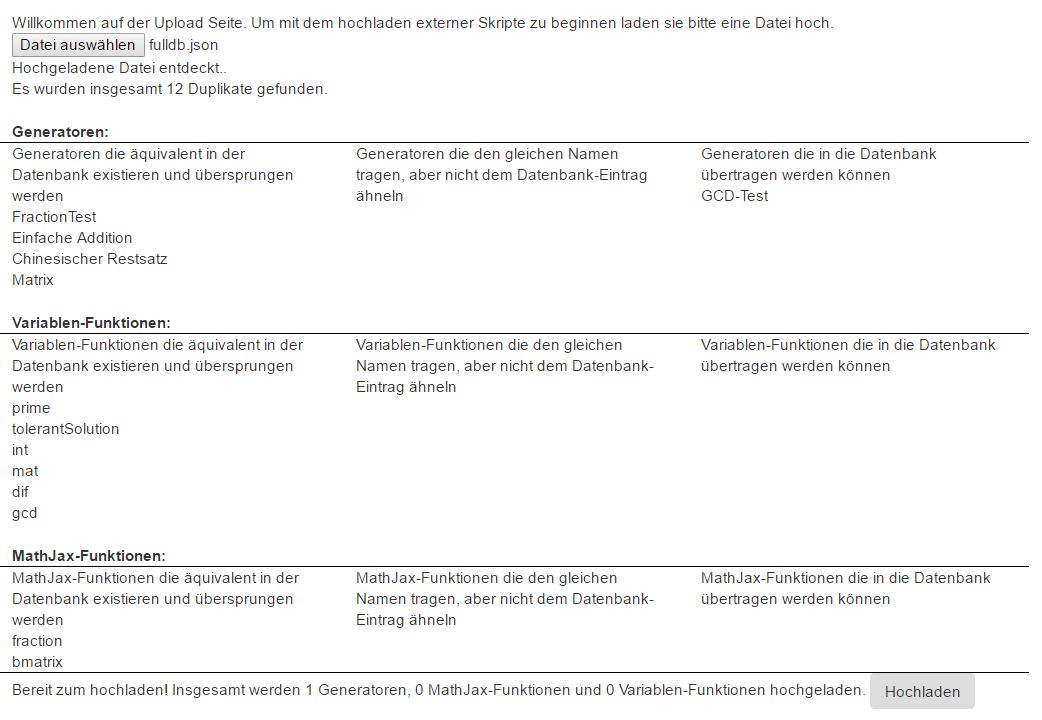
\includegraphics[width=1\textwidth]{bilder/UploadEntities} 
\caption[Ergebnis der Analyse einer Datei]{Ergebnis der Analyse einer Datei}
\end{figure} 

Die Ansicht ist in drei Zeilen aufgespalten, eine für die Generatoren, eine für die Variablen- und eine für die MathJax-Funktionen. Auf der linken Seite werden dem Nutzer alle Datensätze angezeigt, welche äquivalent in der Datenbank existieren und daher nicht hochgeladen werden müssen. Die Mitte dient der Anzeige aller Entitäten die mit der Datenbank in Konflikt treten, während die rechte Seite der Anzeige der Entitäten dient, welche hochgeladen werden können. \\

Für die Anzeige dieser Seite gibt es drei Fälle.\\

\noindent \textbf{1.Es wurden keine Einträge in der Datenbank gefunden die nicht bereits existieren } \\
In diesem Fall werden lediglich die Duplikate in der linken Spalte angezeigt. Am unteren Ende der Seite erscheint ein Info-Text, dass die Datei keine Neuerungen enthält. \\

\noindent \textbf{2.Eine oder mehrere Entitäten kollidiert mit einem bereits existierenden Eintrag in der Datenbank } \\
Der Info-Text zeigt eine Information an, dass der Upload-Prozess nicht fortgesetzt werden kann, da ein Konflikt mit der Datenbank besteht. \\

\noindent \textbf{3.Es wurde kein Konflikt festgestellt und die Datei enthält nicht ausschließlich Duplikate} \\
Bei diesem handelt es sich um den Fall der für den Nutzer wünschenswert ist. Er bekommt die Information, dass der Upload bereit ist, sowie die Zusammenfassung wie viele Generatoren / Mathjax-Funktionen und Variablen-Funktionen bei Starten des Prozesses hochgeladen werden. Der Knopf zum Starten des Upload-Prozesses wird dargestellt. Sobald dieser gedrückt wird, wird ein Datensatz mit allen Entitäten die in die Datenbank aufgenommen werden abgeschickt. Wichtig ist hierbei zu sagen, dass keine doppelten Entitäten abgeschickt werden.\\



\subsection{Der Fehler-Log}

Eine wichtige Frage bei der Entwicklung einer Anwendung ist immer die Frage was alles schief gehen kann. Welche Fehler können auftreten und wie können sie behandelt oder sogar umgangen werden? \\
Einer der Hauptfehler der bei OpenTasks auftreten kann sind Fehler während der Generierung der Aufgaben. Da diese Skripte vom Nutzer geschrieben werden sind die Möglichkeiten diese zu überprüfen stark beschränkt. Eine der Möglichkeiten ist natürlich sie mehrmals laufen zu lassen und zu überprüfen ob ein Fehler zur Laufzeit erzeugt wird. Allerdings besteht hier immer die Gefahr, dass der Fehler der erzeugt wird genau bei diesen Testläufen nicht auftritt. Somit kann nie garantiert werden, dass alle Generatoren die sich in der Datenbank befinden korrekt sind und zur Laufzeit keine Fehler erzeugen. Die einzige Sache die durch solch empirische Tests gezeigt werden kann ist, dass die Wahrscheinlichkeit, dass die Generierung funktioniert recht hoch ist. \\

Was ist nun aber die Lösung für dieses Problem? In der Implementierung wird so vorgegangen, dass immer eine Aufgabe erzeugt wird. Sollte dieser Prozess fehlschlagen wird ein Fehler produziert. Dieser Fehler wird zum einen an den Nutzer (den Studenten) weitergeleitet und auf seiner Seite angezeigt. Zusätzlich wird jeder Fehler der registriert wird auf Server-Seite abgespeichert. Der Administrator hat nun die Möglichkeit in der Webanwendung auf den Tab ``Fehler-Log'' zu gehen. Sobald diese Seite besucht wird wird eine Anfrage an den Server gesendet. Dieser antwortet mit einem Datensatz der alle Fehler enthält die während der Laufzeit produziert wurden. Daraufhin könnnen diese evaluiert und der entsprechende Generator korrigiert werden, sodass dieser Fehler in Zukunft vermieden werden kann. \\

Die zweite Fehlerquelle ist die Validierung der Skripte. Da auf Server-Seite ebenfalls eine Validierung der Skripte statt findet (siehe Kapitel \ref{GenerateTaskChapter} Die Sicherung der Aufgaben-Generierung) müssen die Fehler die hier entdeckt werden für den Administrator sichtbar sein. Diese werden ebenfalls in dem Fehler-Log angezeigt und können dort nachgelesen werden.

\begin{figure}[htp]     % h=here, t=top, b=bottom, p=page
\centering
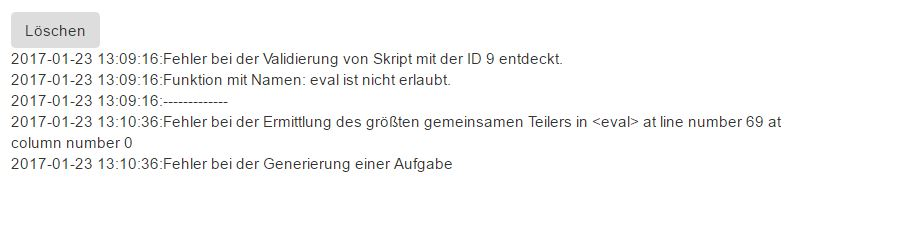
\includegraphics[width=1\textwidth]{bilder/ErrorLog} 
\caption[Der Fehler-Log]{Der Fehler-Log}
\end{figure} 




\chapter{Ein Blick unter die Haube - das Backend}




\section{Die JavaScript-VM}

Bevor auf die Frage eingegangen wird wie die Nutzung von JavaScript-Code in einem Java-Server umgesetzt wurde ist zuerst eine andere Frage offen: Warum muss eigentlich JavaScript-Code ausgeführt werden? \\

Es stand fest, dass der Administrator in der Lage sein muss eigene Skripte zu schreiben. Dadurch konnte gewährleistet werden, dass auch Aufgaben generiert werden können an die bei der Erstellung des Programmes nicht gedacht werden konnte. \\
Damit der Administrator Skripte schreiben konnte musste also eine Sprache gefunden werden, die folgende Bedingungen erfüllt:
\begin{enumerate}
\item Die Sprache sollte möglichst weit verbreitet sein. So wird kein Zwang erzeugt nur für diese Anwendung eine Sprache zu lernen.
\item Die Sprache sollte entweder Java selbst sein oder innerhalb von Java ohne großen Aufwand ausgeführt werden können.
\end{enumerate}

Bei der Recherche hat sich gezeigt, dass sich JavaScript zu einer äußerst populären Sprache entwickelt hat. Da es sich bei JavaScript zusätzlich um eine Sprache mit sehr leichter Syntax handelt und sie sich zusätzlich sehr leicht in Java-Code integrieren lässt ist die Wahl auf JavaScript gefallen. \\

Die Skripte selber werden aus den Skript-Entitäten erzeugt. Ein fertiges Skript besteht immer aus vier Funktionen. Die ersten drei sind vom Administrator geschrieben und sind für die Erzeugung der Variablen/des MathJax und der Validierung der Lösung zuständig. Als vierte Funktion existiert die Funktion die im MathJax die Variablen einsetzen.\\

\emph{Java-Code zur Erstellung eines Generator-Skripts}
\begin{lstlisting}
public String constructScript(ScriptEntity entity) {
	StringBuilder builder = new StringBuilder();
	builder.append("function generateVariables() {");
	builder.append(entity.getVariableScript());
	builder.append("}");
	builder.append("function generateMathjax(variables){");
	builder.append(entity.getMathjaxScript());
	builder.append("}");
	builder.append("function testSolution(variables, userinput) {");
	builder.append(entity.getSolutionScript());
	builder.append("}");
	builder.append("function getComputedMathjax(variables){");
	builder.append("var mathjax= generateMathjax(variables);");
	builder.append("for (var key in variables) {");
	builder.append("var replacer = \"$\" + key;");
	builder.append("mathjax = mathjax.split(replacer).join(variables[key]);");
	builder.append("}");
	builder.append("return mathjax");
	builder.append("}");	
	String script = builder.toString();
	return script;
}
\end{lstlisting}

Das Generator-Skript ist allerdings nicht der einzige Code der geladen werden muss. Die Helper-Methoden müssen ebenfalls geladen werden, da die Generatoren ansonsten nicht funktionieren können. \\

\emph{Java-Code zur Erstellung der Helper-Funktionen}
\begin{lstlisting}
public String getMathjaxScript() {
	StringBuilder builder = new StringBuilder();
	builder.append("mj= { \n");
	appendScript(mjRepo.findAll(), builder);
	builder.append("\n}");
	return builder.toString();
}

public String getVariableScript() {
	StringBuilder builder = new StringBuilder();
	builder.append("vf= { \n");
	appendScript(vfRepo.findAll(), builder);
	builder.append("\n}");
	return builder.toString();
}

private void appendScript(Iterable<? extends FunctionEntity>entities, StringBuilder builder) {
	boolean appendComma=false;
	for (FunctionEntity entity : entities) {
		if(appendComma) {
			builder.append(", \n");
		}
		if(entity.getConstants()!=null) {
			builder.append(entity.getConstants());
			builder.append(",\n");
		}
		builder.append(entity.getName()+":function(");
		builder.append(entity.getParams());
		builder.append("){\n");
		builder.append(entity.getCode());
		builder.append("}");
		appendComma=true;
	}
}

\end{lstlisting}

Die hier erstellten Code-Schnipsel werden zusammengefügt und bilden so das gesamte Skript, welches in die virtuelle Maschine geladen wird. Dafür wurde ein Service erstellt, welcher die virtuelle Maschine verwaltet und die Schnittstelle zwischen Java und JavaScript bildet. Jede Anfrage die an die JavaScript-VM geht wird über den Service gestellt, welcher diese weiter an die VM stellt.\\

\emph{Beispiel für die Validierung einer Aufgabe}
\begin{lstlisting}
public boolean validateAnswer(Bindings variables, String answer) throws ScriptException {
	try {
		return (boolean) invocable.invokeFunction("testSolution", variables, answer);
	} catch (NoSuchMethodException e) {
		throw new RuntimeException(e);
	}
}
\end{lstlisting}

\section{Die Sicherung der REST-API}

Ein wichtiger Punkt bei der Entwicklung eines Backends ist immer die Sicherheit. Daher wird in diesem Kapitel darauf eingegangen wie in dieser Applikation die Sicherheit der REST-API, sowie die zusätzliche Sicherheit die auf dieser Seite für den Nutzer eingebaut wurde, erreicht wurde. \\


\subsection{Authentifizierung und Rollen-System}

TODO: Rollen und zugehörige Authorities beschreiben

Eine der grundlegenden Fragen wenn es um Sicherheit geht ist die Authentifizierung. Für diese Anwendung wurden \hyperref[JWT]{JSON Web Tokens} gewählt um eine Authentifizierung zu gewährleisten. \\
In der Implementation bedeutet dies, dass bevor der erste Austausch von Nutzdaten erfolgen kann als erstes der Austausch des Tokens erfolgen muss. Von der Seite des Nutzers wird eine Anfrage gesendet welche Nutzername und Passwort beinhaltet. Dieses wird mit der Datenbank abgeglichen. Wird der Nutzer gefunden und ist das Passwort korrekt wird ein Token generiert und an den Anfrage-Steller zurück gesendet. Wichtig ist hierbei zu erwähnen, dass die Passwörter nur in kodierter Form in der Datenbank vorliegen (für diese Anwendung wurde als Kodierung der Algorithmus MD5 gewählt) und so gewährleistet wird, dass wenn ein fremder Lesezugriff auf die Datenbank auftreten sollte die Passwörter schwerer zu entschlüsseln sind. \\
Jedes mal wenn nun Daten abgefragt werden sollen schickt der Nutzer sein Token mit. Der Server überprüft die Validität des Tokens und wenn diese gewährleistet wurde erhält der Nutzer die angefragten Daten. \\

Allerdings ist dies nicht der einzige Mechanismus der in der REST-API eingebaut wurde. Jeder Nutzer hat eine Rolle welche in der Datenbank eingespeichert ist. Bei der Authentifizierung wird ebenfalls die Rolle dieses Nutzers ausgelesen. Jede Rolle hat einen fest zugewiesenen Satz an Befugnissen, welche bei dem Authentifizierungsprozess aus der Datenbank geladen und dem Nutzer angehängt werden. \\
Der Großteil der Controller hat als Voraussetzung um die Daten abfragen zu dürfen vorher eine Abfrage ob die Person die aktuell die Daten anfragt die benötigte Befugnis besitzt diese zu lesen. Ist diese Abfrage erfolgreich werden die Daten ausgeliefert, ansonsten kommt als Antwort lediglich ein 403 - Forbidden. \\

Für den Studenten wurde hierbei ein Account eingerichtet, welcher von allen benutzt wird und nur die Rechte besitzt um auf alle Endpunkte zuzugreifen die für Erhalt und Bearbeitung der Aufgaben von Nöten sind. \\

Für den Administrator kann es allerdings beliebig viele Accounts geben. Diese können alle in der Datenbank eingetragen und genutzt wurden. Dies muss allerdings alles direkt auf der Datenbank-Ebene geschehen, da es keine Seite gibt die diese Funktion abdeckt.

\subsection{Die Sicherung der Aufgaben-Generierung}\label{GenerateTaskChapter}

Neben der Sicherung der Rest-API an sich ist natürlich ein weiterer wichtiger Aspekt die Sicherung der Aufgaben-Generierung. Einerseits muss darauf geachtet werden, dass sich kein unerlaubter Code auf der Seite des Servers befindet und hier Schaden anrichten kann, andererseits ist es ebenfalls wichtig, dass keine Entitäten an den Administrator ausgeliefert werden die schadhaften Code enthalten (wenn er die Generatoren editiert und dabei auch testet). \\

Um dies zu bewerkstelligen wurde ein Ansatz gewählt, welcher in der selben Implementation im Frontend existiert.. Jeder Generator, sowie jede Helper-Funktion, wird an verschiedenen Stellen getestet. Bei dem Backend ist dies der Fall wenn der Administrator eine Entität bearbeitet hat und persistieren will, auf der Seite des Frontends wird jedes Mal getestet bevor der Code validiert und in den Arbeitsspeicher geladen wird. Dabei wird darauf geachtet welche Funktionsaufrufe getätigt wurden. \\

Für die Validierung existiert eine Liste von erlaubten Funktionen auf der Server-Seite. Um diese Liste zu erstellen werden als erstes alle existierenden Helper-Funktionen aus der Datenbank geladen. Der Name von jeder wird der Liste von erlaubten Funktionen hinzugefügt. Abschließend gibt es in der Konfiguration der Anwendung noch die Möglichkeit über die application.properties Funktionen einzutragen welche zusätzlich erlaubt werden sollen. \\

Nachdem diese Liste erstellt wurde wird sie mit den Namen aller in dem Skript aufgerufenen Funktionen verglichen. Sollte eine Funktion gefunden werden, welche nicht erlaubt ist führt dies zu einem Fehler. Auf Seite des Servers bedeutet dies, dass die Entität nicht gespeichert wird und dem Sender der Speicher-Anfrage ein Fehler zurück gegeben wird. In dem Frontend wird dem Nutzer angezeigt, dass nicht erlaubte Funktionen gefunden wurden, sowie die Namen dieser angezeigt. \\

Gleichzeitig wirft dieser Prozess eine Frage auf: Welchen Mehrwert hat es Code zweimal zu testen, beide Male mit der selben Methode? Um diese Frage zu beantworten ist es wichtig sich folgendes bewusst zu machen: Der Code auf der Client-Seite kann korrumpiert werden. Ein Nutzer mit dem Ziel Schaden zuzufügen könnte ihn editieren und so Anfragen schicken, welche normalerweise direkt auf Client Seite abgefangen und verboten werden würden. Sollte der Code allerdings nicht korrumpiert sein, so ist gute Praxis einen Generator bevor er abgeschickt wird zu testen, so wird der unnötige Austausch von Daten vermieden und dem Nutzer insgesamt eine flüssigere Erfahrung geboten. Zusätzlich wird die Server-Last reduziert da dieser weniger testen muss.


\section{Dokumentation der REST-Schnittstellen}

\subsection{Admin}

Benötigte Befugnis : ADMIN \\

\noindent Pfad: admin/generators \\
Methode: GET \\
Beschreibung: Sucht alle Generatoren und gibt ihre Namen zurück \\
Rückgabe: \begin{lstlisting} 
["Euklidischer Algorithmus", "Matritzenmultiplikation"]
\end{lstlisting}

\noindent Pfad: admin/generator \\
Methode: GET \\
Beschreibung: Sucht den Generator mit dem angegebenen Namen und gibt ihn zurück \\
URL-Parameter: name : Der Name des Generators \\
Rückgabe: \begin{lstlisting} 
{
  "id": 19,
  "name": "Einfache Addition",
  "variableScript": "var a = vf.int(10,20)\nvar b = vf.int(10,20)\nvar solution = a+b\nreturn {a:a, b:b, solution:solution}",
  "solutionScript": "return variables.a + variables.b = solution",
  "mathjaxScript": "return \"$$ $a + $b $$\"",
  "formType": "Numbers"
}
\end{lstlisting}

\section{Die Kommunikation mit den Administratoren}

Wenn man über die Features im Frontend nachdenkt bleibt man an einer Sache hängen: Die Übersicht über die laufende Aufgabe. Auf dieser Seite erhält der Administrator jederzeit den aktuellen Stand über die Punktzahl der verschiedenen Teams. Doch wie wurde dies umgesetzt? \\

Für die Implementation wurde auf die in der Einleitung erklärten Websockets zugegriffen. Sobald der Administrator auf die Übersicht Seite wechselt sendet er automatisch eine Anfrage an den Server gesendet um eine Websocket-Verbindung zu öffnen. Der Server nimmt automatisch jede Anfrage an. \\
Sobald der Client die Rückmeldung bekommt, dass die Authentifizierung erfolgreich war sendet er seine Daten zum einloggen. Für den Administrator sind das die selben Daten die zum erhalten des Tokens genutzt wurden. Diese werden beim Login-Prozess zwischengespeichert und für diesen Zweck wieder verwendet. \\
Sobald der Server diese Login-Anfrage erhält überprüft er in der Datenbank ob es sich hierbei um eine gültigen Account handelt. Ist dies der Fall wird der Socket in der Liste der autorisierten Administratoren gespeichert. \\

Sobald ein neuer Generator gestartet wird wird gleichzeitig auch eine andere Routine gestartet. Diese wird jede Sekunde ausgeführt und hat nur eine Aufgabe: Die Administratoren über den aktuellen Punktestand informieren. Bei dem ausführen wird der aktuelle Stand in ein Objekt verpackt, welches über den Websocket verschickt wird. Der Administrator analysiert dieses Packet bei Erhalt und aktualisiert die Ansicht entsprechend.


\section{Die Generierung und Validierung der Aufgaben}

Kommen wir zu dem Hauptpunkt der Anwendung. Die Generierung und Validierung der Aufgaben. Jedes Mal wenn ein Generator angefragt wird wird dieser aus der Datenbank geladen. Die hier geladene Entität enthält allerdings nur Bruchstücke des Codes zur Generierung, wobei diese reichen um den Generator eindeutig zu rekonstruieren.\\
Sobald die Rekonstruktion abgeschlossen ist wird eine virtuelle Machine gestartet innerhalb der Code ausgeführt und die Aufgaben generiert werden. Um die virtuelle Machine(VM) zu starten und die Kommunikation zwischen Java und Javascript Code zu ermöglichen wird die Java Scripting API\footnote{https://docs.oracle.com/javase/8/docs/technotes/guides/scripting/prog_guide/api.html} genutzt, auf die hier nicht weiter eingangen wird. \\

Sobald der Generator geladen wurde wird eine Rückmeldung an die Routine gegeben die ihn gestartet hat. Kommt nun eine Anfrage an den Server eine Aufgabe zu generieren wird dies an die Javascript-VM weitergeleitet. Der dafür benötigte Kontext wird hierbei der eindeutigen ID des Nutzers zugeordnet und abgespeichert. Bei erfolgreicher Generierung wird die generierte Aufgabe zurück gegeben, damit sie vom Nutzer bearbeitet werden kann. Sollte während der Generierung ein Fehler auftreten so wird dieser in den Fehler-Log geschrieben, damit er vom Administrator eingesehen werden kann. Der Nutzer bekommt in dem Falle lediglich die Rückmeldung, dass während der Generierung seiner Aufgabe ein Fehler aufgetreten ist. Sollte es sein Wunsch sein kann er daraufhin ein weiteres Mal eine Aufgabe anfordern. \\

Sobald die Aufgabe bearbeitet und die Lösung zum Server geschickt wurde wird als erstes überprüft ob überhaupt ein Generator aktiv ist. Sollte keiner aktiv sein wird dem Nutzer zurückgemeldet, dass die Bearbeitungszeit bereits abgelaufen ist. Ansonsten wird die eindeutige ID des Nutzers aus dem Token, welches er zur Authentifizierung genutzt hat ausgelesen. Diese ID wird nun genutzt um den Kontext der Aufgabe zu finden. Hier bestehen nun zwei Fälle. \\

1. Es wurde kein Kontext für die ID des Nutzers gefunden.\\
Dies ist immer dann der Fall wenn seit dem Erhalt der Aufgabe ein neuer Generator gestartet wurde. Sobald ein neuer Generator gestartet wird wird jedes Mal die Liste von allen momentan gespeicherten Kontexten gelöscht und eine neue angelegt. \\

2. Der Kontext wurde gefunden.\\
In diesem Fall kann mit der Validierung der Aufgabe begonnen werden. Der JavaScript-VM wird der Kontext(die Variablen, welche bei der Generierung genutzt wurden), sowie die Antwort des Nutzers übergeben. Diese validiert nun die Korrektheit der Antwort und gibt entsprechend true oder false an den Java-Teil der Anwendung zurück. \\
Wenn die Antwort als korrekt befunden wurde wird eine neue Aufgabe generiert, der Kontext wieder unter der ID des Nutzers abgespeichert und die Aufgabe zurück gesendet. Zusätzlich wird seinem Team eine korrekt gelöste Aufgabe zugeschrieben und alle verbundenen Administratoren über den neuen Punktestand informiert. \\
Sollte die Aufgabe allerdings falsch gelöst worden sein wird keine neue Aufgabe generiert. Stattdessen wird dem Team des Nutzers eine falsch gelöste Aufgabe zugeschrieben (und alle verbundenen Administratoren informiert). An den Nutzer kommt lediglich die Rückmeldung, dass die Antwort falsch war.

\chapter{Fazit}




\section{Das Ergebnis}

Rückblickend lassen sich mehrere Erkenntnis aus der Entwicklung und dem Produkt das Open Tasks geworden ist ziehen. \\

Eine der größten Erkenntnisse ist wie schwer es ist zu verhindern, dass schadhafter Code in ein Programm eingeschleust wird in dem es dem Nutzer erlaubt wird selber Skripte zu schreiben. Immer wieder sind große Hindernisse in den Weg gekommen oder große Lücken aufgefallen durch die sich doch etwas einschleusen lässt, die allerdings nicht ohne weiteres zu beheben waren. Daher ist es in der Endversion von Open Tasks so, dass die vom Administrator erzeugten Skripte nicht auf unerlaubte Funktionen überprüft werden. Die alte Funktionalität ist noch da, da sie allerdings der vollen Funktionalität von Open Tasks schadet wurde sie zeitweise deaktiviert. \\
Das bedeutet, dass die einzige Sicherheit die momentan existiert darin besteht, dass nur der Administrator einen gesicherten Zugriff auf die Editierung der Skripte erhält. \\

Ein weiterer großer Punkt war die Zerteilung des Programmes in mehrere logische Einheiten um die Komplexität zu senken. Es stellte sich als nicht trivial heraus dies zu tun ohne, dass mehr Kommunikation zwischen diesen logischen Einheiten notwendig war als gewollt, da es viele Einheiten gab die nicht eindeutig zugeordnet werden konnten und sich so teilweise in zwei verschiedenen Abschnitten(Services) des Programmes befanden. \\

Was allerdings erstaunlich gut geklappt hat war die Validierung und Erzeugung der Aufgaben. Als mit der Programmierung von Open Tasks begonnen wurde gab es viele Abschnitte in denen unklar war ob sie funktionieren würden wie sie sollten und dies war ein großer Knackpunkt in der Entwicklung. Tatsächlich ist allerdings ein gut funktionierendes Konstrukt entstanden, welches im Fehlerfall ausführlich Feedback an den Administrator sendet. \\



\section{Wie kann die Anwendung verbessert / erweitert werden}

Doch so viele gute Punkte es bei Open Tasks auch gibt, einige Sachen sind nicht optimal und könnten in einer weiteren Iteration der Entwicklung verbessert werden. \\

Einer der großen Punkte ist das optische Auftreten der Webapplikation. Es wurde bereits relativ viel Arbeit darin gesteckt die Anwendung graphisch ansprechend zu gestalten, doch ist das Ergebnis nicht das Ende aller Möglichkeiten in diesem Bereich. \\
Eine Option in diesem Bereich wäre es einen Grafiker zu engagieren, welcher ein ausführliches Konzept für das Design der Seite erstellt. Sobald es dieses gibt sollte es ein leichtes sein dieses auf der Seite umzusetzen, insbesondere da Angular 2-Anwendungen durch ihre Modularität leicht in einzelnen Abschnitten zu überarbeiten sind.\\
Sollte dies umgesetzt werden würde dies die User-Experience merklich verbessern. \\

Doch nicht nur die Ansicht des normalen Nutzers könnte eine Überarbeitung vertragen. Auch auf der Seite des Administrators gibt es einige Möglichkeiten zur Erweiterung.\\
Eine der wichtigsten Sachen auf dieser Seite ist wohl der Code-Editor. Mit viel Aufwand wäre es möglich hier eine Online-Entwicklungsumgebung einzurichten, folgende Features sind als Vorschläge zu sehen:
\begin{description}

\item -Code-Vervollständigung
\item -Überprüfung von Fehlern zur Übersetzungszeit
\item -Code-Highlighting
\end{enumerate}


Neben den Änderungen am Interface gibt es allerdings auch mehrere Dinge die im Code geändert werden könnten und keinen direkt ersichtlichen Einfluss auf Open Tasks hätten.\\

Zuallererst ist die Test-Ebene zu nennen. Momentan besitzt Open Tasks keine Tests. Dabei ist dies für das Backend, sowie das Frontend der Fall. Angular 2, sowie Spring-Boot bieten ausgezeichnete Möglichkeiten Unit-Tests zu schreiben, doch auch für Integration-Tests gibt es gut dokumentierte Möglichkeiten. \\

Abschließend ist noch das Rollen-System zu nennen. Momentan sind die Rollen und zugehörigen Zugriffsrechte ziemlich hart im Code definiert und nicht ohne Änderung des Codes zu ändern. Sollte die Applikation wachsen könnte sich dies zu einem Hindernis entwickeln. Daher steht es zur Option die Rechte die jeder Rolle zustehen nicht im Code, sondern in der Datenbank zu definieren und dynamisch auszulesen.

\listoffigures
\begin{thebibliography}{}

% Formatierung für Internetquelle
% Grundregel: Name, Vorname (falls vorhanden), Vö-Jahr (falls vorhanden), Titel in Anführungszeichen, URL, Datum des letzten Aufrufs
% zur Formatierung der URL unbedingt den url-Befehl benutzen!!!

\bibitem[Spring Dokumentation(2016)]{spring}
Spring-Dokumentation
\url{https://spring.io/docs}, letzter Zugriff: 17.12.2016

\bibitem[Spring-Boot Dokumentation(2016)]{spring-boot}
Spring-Boot-Dokumentation
\url{http://docs.spring.io/spring-boot/docs/current-SNAPSHOT/reference/htmlsingle/}, letzter Zugriff: 17.12.2016

https://blog.php-dev.info/2014/04/mariadb-vs-mysql/
https://www.quora.com/What-are-the-advantages-and-disadvantages-of-using-Sinatra-vs-Express-for-a-web-service-API
https://medium.freecodecamp.com/angular-2-versus-react-there-will-be-blood-66595faafd51#.ufvfcrtqo


\bibitem[Blu-ray Disc Association(2005)]{bluray} 
Blu-ray Disc Association: 
\emph{White paper Blu-ray Disc Format 2.B Audio Visual Application, Format Specifications for BD-ROM}, 
\url{http://www.blu-raydisc.com/Assets/downloadablefile/2b_bdrom_audiovisualapplication_0305-12955-15269.pdf}, 2005, letzter Zugriff: 1. 10. 2012

https://www.heise.de/developer/meldung/Programmiersprachen-Ranking-JavaScript-und-Java-weiter-an-der-Spitze-3113468.html?view=zoom;zoom=1
https://jaxenter.de/programmiersprachen-rankings-49399

https://www.informatik-aktuell.de/betrieb/datenbanken/mariadb-und-mysql-vergleich-der-features.html
% Formatierung für Aufsatz / Paper: Titel in Anführungszeichen, Zeitschriftentitel kursiv
\bibitem[Dooley \& Streicher(1982)]{dooley_streicher} 
Dooley, Wesley L.  \& Streicher, Ronald D.:
\glqq M--S Stereo: A Powerful Technique for Working in Stereo\grqq, 
\emph{Journ. Audio Engineering Society} vol. 30 (10), 1982

% Formatierung für Fachbuch, Diplomarbeit o.Ä.: Titel kursiv
\bibitem[Kuttruff(1991)]{kuttruff}
Kuttruff, Heinrich: 
\emph{Room Acoustics}, 3. Aufl., Elsevier 1991

% Formatierung für Fachbuch mit Herausgeber und mehreren Autoren
\bibitem[Spehr(2009)]{spehr}
Spehr, Georg (Hrsg.): 
\emph{Funktionale Klänge}, transcript 2009

% Formatierung für ein einzelnes Kapitel eines speziellen Autors aus einem Fachbuch mit mehreren Autoren
\bibitem[Sowodniok(2009)]{sowodniok}
Sowodniok, Ulrike: 
\glqq Funktionaler Stimmklang -- Ein Prozess mit Nachhalligkeit\grqq, 
in: Spehr, Georg (Hrsg.): \emph{Funktionale Klänge}, transcript 2009

% Formatierung für Aufsatz / Paper: Titel in Anführungszeichen, Zeitschriftentitel kursiv
\bibitem[Stephenson(1990)]{stephenson}
Stephenson, Uwe: 
\glqq Comparison of the Mirror Image Source Method and the Sound Particle Simulation Method\grqq, 
\emph{Applied Acoustics} vol. 29, 1990


\end{thebibliography}

%--------------------- EIGENST�NDIGKEITSERKL�RUNG ---------------
\clearpage\thispagestyle{empty}
\eigen  % im header definiert
%--------------------------------------- ENDE ------------------------------------
\end{document}
%%%%%%%%%%%%%%%%%%%%%%%%%%%%%%%%%%%%











